\chapter{Information Retrieval}{
Information Retrieval~\cite{buttcher:2010:IR} (IR) deals with
representing, searching and manipulating large collections of texts. The
Figure~\ref{fig:IR} depicts the components of an IR system. By issuing a
\emph{query} which consists in a group of \emph{keywords} (i.e., index terms)
to an IR system, a user expresses his need for information to the machine, i.e.
the \emph{information need}. A \emph{term} is not necessarily a word, but can
also be a phrase, a date or any other set of words. The machine task is to
return a set of documents that are useful, i.e., \emph{relevant}, to the user
in some sense. A returned document is given a \emph{score} with regards to the
issued query, that indicates how much relevant the document is to the query.
This way returned results can be \emph{ranked} with regards to their scores.

The use of IR services is now widespread thanks to web search engines such as
Google of Bing. Users of such services expect it to return up-to-date, accurate
and near-instantaneous answers to a query. \cite{baeza-yates:2007:icde} reports
that IR web search engines are still able to give good performance even at the
web scale, which contains billions of documents. In order to achieve a
sub-second response to the user, web search engines do not only rely on hardware
performance, but also on the efficiency of data structures and other models that
it will use.

A major task of a search engine is to maintain and manipulate an \emph{inverted
index} for a document collection. This data structure is the main structure
used by a search engine for searching and ranking. As a basic function, the
inverted index provides a mapping between the terms and the locations in the
documents in which they occur. Terms' Locations are stored into a data
structure called \emph{inverted lists}. The size of inverted lists are on the
same magnitude as the collection itself. Thus search and retrieval operations
must be done with care in order to be efficient.

\begin{figure}
\centering
\resizebox{0.7\linewidth}{!}{%
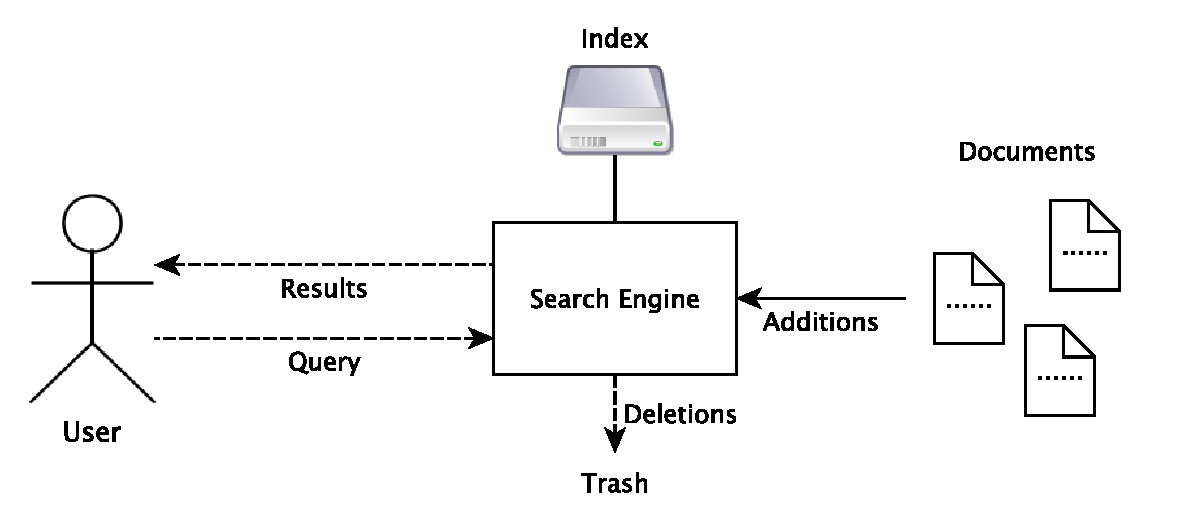
\includegraphics[scale=1]{pics/IR}
}%
\caption{Principal components of an IR system.}
\label{fig:IR}
\end{figure}
}
\label{chap:IR}
\section{Inverted Index}
\label{sec:inverted-index}

An index can be seen as a matrix with the terms (e.g. unigram) for rows and the
collection's documents as columns. In this matrix, an element
equal to one if the term i occurs in document j, and zero if not. However such
a matrix contains practically only zeros, thus a lot of wasted space. Inverted
List is a basic IR structure that reduces such a matrix to only store ones'
values. All the inverted lists taken together form the inverted index.

From the collection a dictionary of the words appearing in is created. The
dictionary's terms have been first filtered, by removing the punctuation for
example. Given a term from the dictionary, a linked list is associated to it
and stores all documents records where the term occurs in. A document record
can be simply a serial number of the document (i.e., document identifier), but
additional information like the term frequency and the position can be given.
The term frequency corresponds to the number of occurrences of the term in a
document, and the position indicate the positions of the occurrences within
that document. The Figure~\ref{fig:inverted-list} depicts two inverted lists
storing documents identifiers as integers, term frequencies and positions.
These inverted lists are built using the terms ``killed'' and ``brutus'' from
documents in the Table~\ref{tab:indexing}. There
is a relation one-to-one between documents identifiers and term frequencies,
and a relation many-to-many with the positions. There are as much position
values as there are occurrences (i.e., term frequency) of the term in the
document. The documents identifiers are stored in increasing order in order
to process queries, as presented in Section~\ref{sec:query-model}.

\begin{figure}
\centering
\resizebox{0.8\linewidth}{!}{%
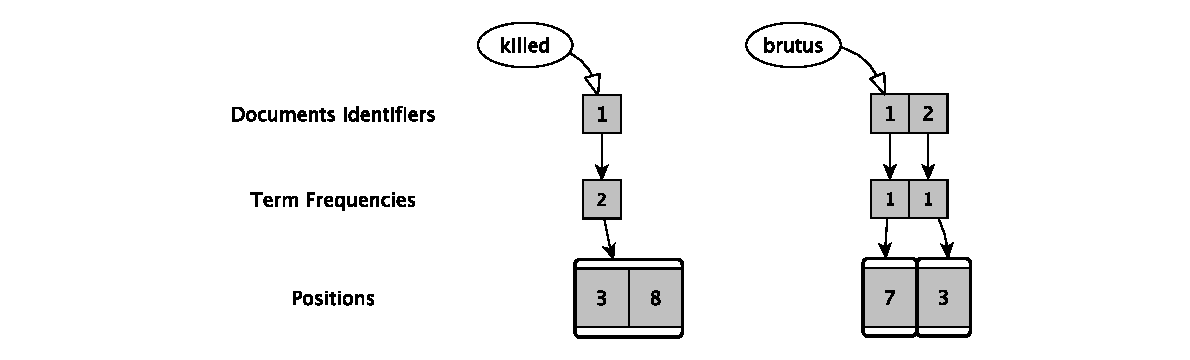
\includegraphics[scale=1]{pics/inverted-list}
}%
\caption{Inverted lists for the terms ``killed'' and ``brutus'' in documents
from the Table~\ref{tab:indexing}. Each inverted list stores the documents
identifiers, the term frequencies and the positions information.}
\label{fig:inverted-list}
\end{figure}

\subsection{Indexing}
\label{sec:IR-indexing}

In this section, traditional inverted index construction is presented, then the
block-based construction which makes possible to handle large collection.
Finally I discuss the importance of compression for large collection, and
present a commonly used  in Information Retrieval encoding technique.

An inverted index is the group of inverted lists built from a collection.
The basic steps to create an inverted index in the main memory from a collection
of documents are:
\begin{enumerate}
  \item make a first pass through the collection to gather term-document-i~dentifiers pairs
  \item sort the pairs with the term value as the key
  \item group together docIDs of a same term into an inverted list.
\end{enumerate}
These steps are reported in Table~\ref{tab:indexing} with two documents taken
from the ``Shakespeare's Collected Works'', storing only the document
identifier (docID) in the inverted lists and the document frequency (DF), i.e.
the number of documents the term appears in. Each words in the documents are
filtered by removing the punctuation and lowering the case. The set of terms
defines the dictionary of the inverted index. For each of the dictionary, an
inverted list is then created.

In order to build an inverted index once and for all, the in-memory
inverted index is written to the disk into what is called an \emph{inverted
file}. The Figure~\ref{fig:indexing} summarize the steps from the
collection to the creation of an inverted file. The inverted file contains all
the inverted lists, written one after the other. The dictionary is also stored
in that same file, where each term possess information about the inverted list
it points to: the inverted list's offset or the document frequency, i.e., the
number of documents the term appears in.

\begin{table}
\resizebox{\linewidth}{!}{%
\begin{tabular}{lrllrlllcl}
\toprule
\multicolumn{5}{l}{
{\bfseries Document 1:}
I was killed i' the Capitol; Brutus killed me.
}&
\multicolumn{5}{l}{
{\bfseries Document 2:}
The noble Brutus hath told you Caesar was ambitious.
}\\
\multicolumn{10}{c}{\phantom{a}}\\
{\bfseries term} & {\bfseries docID} & & {\bfseries term (sorted)} & {\bfseries
docID} & & {\bfseries term} & {\bfseries DF} & & {\bfseries Inverted List}\\
I & 1 & \multirow{18}{*}{$\Longrightarrow$} & ambitious & 2 &
\multirow{18}{*}{$\Longrightarrow$} & ambitious & 1 & $\mapsto$ & $1$ \\
was & 1 & & brutus & 1 & & brutus & 2 & $\mapsto$ & $1 \rightarrow 2$ \\
killed & 1 & & brutus & 2 & & capitol & 1 & $\mapsto$ & $1$ \\
i' & 1 & & capitol & 1 & & caesar & 1 & $\mapsto$ & $1$ \\
the & 1 & & caesar & 2 & & hath & 1 & $\mapsto$ & $1$ \\
capitol & 1 & & hath & 2 & & I & 1 & $\mapsto$ & 1 \\
brutus & 1 & & I & 1 & & i' & 1 & $\mapsto$ & $1$ \\
killed & 1 & & i' & 1 & & killed & 1 & $\mapsto$ & $1$ \\
me & 1 & & killed & 1 & & me & 1 & $\mapsto$ & $1$ \\
the & 2 & & killed & 1 & & noble & 1 & $\mapsto$ & $1$ \\
noble & 2 & & me & 1 & & the & 2 & $\mapsto$ & $1\rightarrow 2$ \\
brutus & 2 & & noble & 2 & & told & 1 & $\mapsto$ & $1$ \\
hath & 2 & & the & 1 & & you & 1 & $\mapsto$ & $1$ \\
told & 2 & & the & 2 & & was & 2 & $\mapsto$ & $1 \rightarrow 2$ \\
you & 2 & & told & 2 & & & & \\
caesar & 2 & &  you & 2 & & & & \\
was & 2 & & was & 1 & & & & \\
ambitious & 2 & & was & 2 & & & & \\
\bottomrule
\end{tabular}
}%
\caption{Inverted index creation from two documents taken in ``Shakespeare's
Collected Works''. Each word is filtered and associated to its document
identifier (docID). After sorting the pairs on the term, the inverted lists are
created for the set of terms. The inverted lists store only the docID of the
document the term appears in.}
\label{tab:indexing}
\end{table}

\begin{figure}
\centering
\resizebox{0.8\linewidth}{!}{%
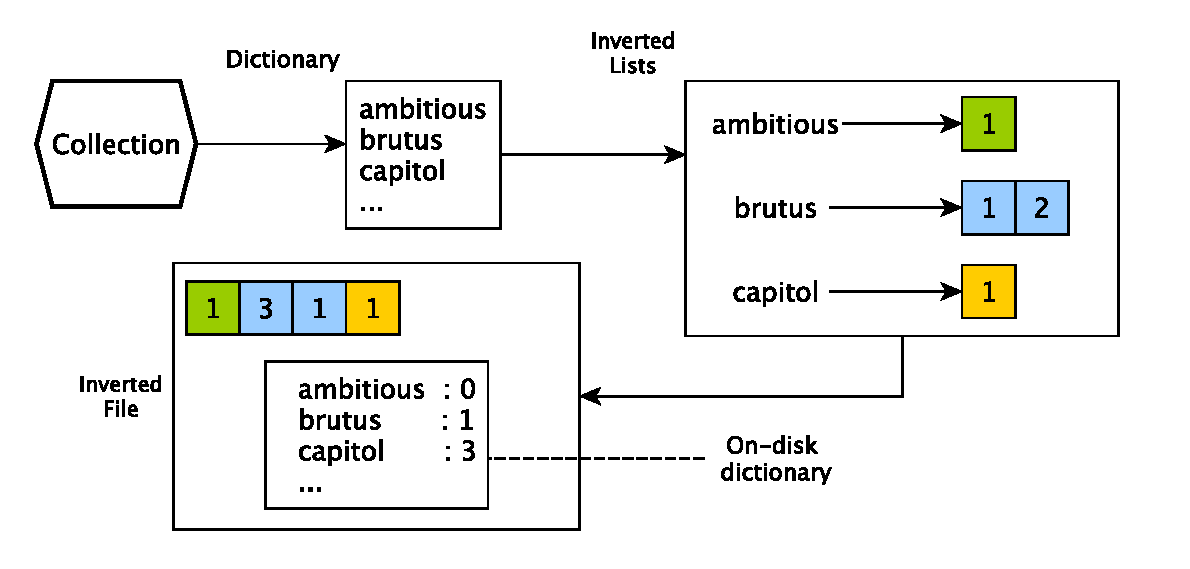
\includegraphics[scale=1]{pics/indexing}
}%
\caption{Indexing, from a collection of documents to the inverted file. The
in-memory inverted lists are written to disk one after the other. The
terms of the embedded dictionary possess offset to the associated inverted list
in the file.}
\label{fig:indexing}
\end{figure}

\subsubsection{Merge-Based Indexing}

The previous indexing technique works in-memory, and then cannot handle large
collection with large inverted lists. Merge-based indexing is a technique that
divides an inverted index construction into segments, which are then merged
together to form a complete inverted index. Thus an inverted list can span
over multiple segments. When the main memory is filled or that a threshold has
been reached, a segment is written to a secondary storage space (e.g. the disk)
into an inverted file. Each on-disk inverted file contains an inverted index
independent from the one in an other segment. When merging inverted files, it is
then necessary to update inverted lists of a same term but stored in different
segments. The Figure~\ref{fig:merged-indexing} depicts the merge process of
three inverted files into one. An inverted list spans over these files: the
documents identifiers values are then local to each file. Thus it is necessary
to update these identifiers numbers in order to keep an ordered inverted list
after merging.

Such an index construction requires two steps to finish. The first one consists
in building multiple segments and is called the \emph{commit} step. The second
one consists in the merging process of multiple files into one inverted file
and is called the \emph{optimization} step. These steps are believed to
be a common operation for incremental inverted index.

\begin{figure}
\centering
\resizebox{0.8\linewidth}{!}{%
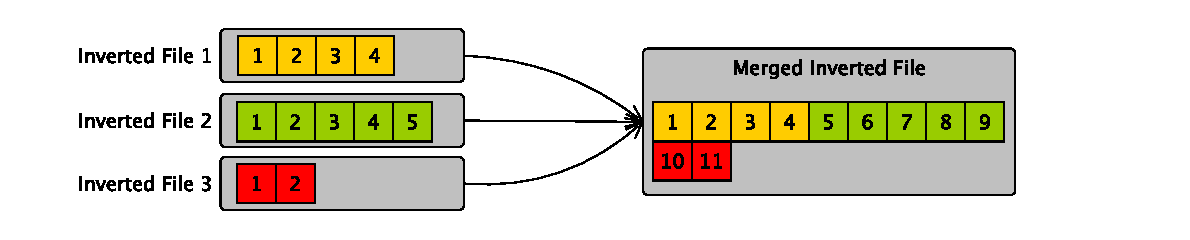
\includegraphics[scale=1]{pics/merged-indexing}
}%
\caption{Merge-based indexing of three inverted files. An inverted list, storing
documents identifiers, spans over these files. When merging these files into
one inverted file, the documents identifiers are updated to keep an ordered
list.}
\label{fig:merged-indexing}
\end{figure}

\subsubsection{Block-Based Inverted List}
\label{sec:compression:block}

For performance and compression efficiency, it is best to store separately each
data stream of an inverted list~\cite{anh:2006:siohttq}. In a non-interleaved
index organisation, the inverted index is composed of three inverted files,
one for each stream of values (i.e., documents identifiers, frequencies and
positions). Each inverted file stores contiguously one type of list, and three
pointers are associated to each term in the lexicon, one pointer to the
beginning of the list in each inverted file.

An inverted file is partitioned into blocks, each block containing a fixed
number of integers as shown in Figure~\ref{fig:index-structure}. Blocks are
the basic units for writing data to and fetching data from disk, but also the
basic data unit that will be compressed and decompressed. A block starts with
a block header. The block header is composed of the length of the block in
bytes and additional meta-data information that is specific to the compression
technique used. Long inverted lists are often stored across multiple blocks,
starting somewhere in one block and ending somewhere in another block, while
multiple small lists are often stored into a single block. For example, 16
inverted lists of 64 integers can be stored in a block of 1024 integers.

\begin{figure}
  \centering
	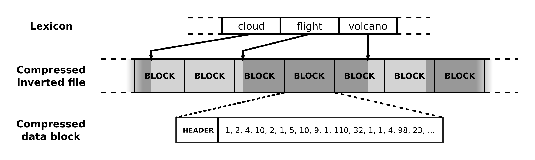
\includegraphics[scale=1.2]{pics/index-structure}
	\caption{Inverted index structure. Each lexicon entry (term) contains a
	pointer to the beginning of its inverted list in the compressed inverted
	file. An inverted file is divided into blocks of equal size, each block
	containing the same number of values.}
	\label{fig:index-structure}
\end{figure}

\subsubsection{Index Updates Strategies}

Updating the inverted index with new documents is done via two approaches: by
\emph{batches} or \emph{incrementally}.
The update strategy by batches stores
added documents into a buffer, and writes them to the index on-disk when some
threshold is reached. While this is adapted to static indexes, in other words
indexes that do not need to be updated right away. However in some cases such
as Internet news search engines, the user would expect the index to be updated
as soon new documents are detected. This use case is matched by incremental
updates strategy. With this strategy, the index is composed of the ones on
disk, but also with an index built in-memory. This second index holds the
updated documents temporarily that are bound to be written to the index on-disk
when a threshold is reached.
The question of deleted documents is handled thanks to a table that stores the
documents flagged in deleted state.

\subsection{Delta-Encoding}

Large collections result in large inverted files. As these files are stored on
disk, compressing their data is then crucial in order to save storage space.
\emph{Delta-encoding} is a basic encoding commonly used in Information
Retrieval which aims to decrease the size of inverted lists, thus reducing
inverted files disk space.

With an ordered and increasing list of integers, it is possible to considerably
reduce the size by storing not the actual integers values but the gaps. A gap
is the difference between two consecutive integers. As the list is increasing,
the difference between an integer at position $i$ and an integer at position
$i-1$ will always be positive. To decompress a value at position i from a
delta-compressed list, we just have to sum up every values up to i. The
Figure~\ref{fig:delta-encoding} depicts a delta-compressed list of integers. By
storing gaps values, we can reduce the size of the list from 88 to 38 bits.

Documents identifiers are stored in increasing order in each inverted list, and
can then be delta-encoded. Also the positions values are stored in increasing
order, but they are local to a document. Thus position values relative to a
same document are delta-encoded, and the encoding is re-initialized when
changing documents.

\begin{figure}
\centering
\resizebox{0.8\linewidth}{!}{%
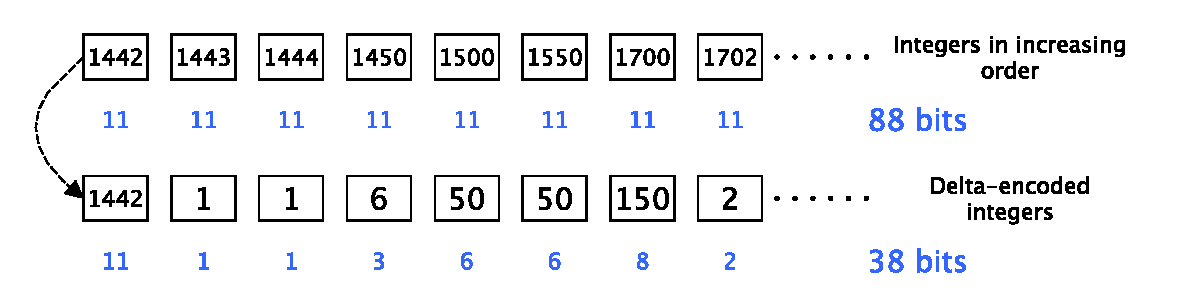
\includegraphics[scale=1]{pics/delta-encoding}
}%
\caption{Delta-encoding of an increasing ordered list of integers, showing the
size in bits of the two lists.}
\label{fig:delta-encoding}
\end{figure}

\section{Query Model}
\label{sec:query-model}

A query is an user request for information about the collection. Documents
matching that query are returned back to the user. In this section, I present
the query model used in Information Retrieval and explain how keyword and
Phrase queries are processed.

The model used to represent documents is the \emph{vector space model},
commonly called the ``bag of words'' model. In this model documents and
queries are seen as vectors, where a component represent a term in the
collection. Given a query and a set of document vectors, we compute the angle
between them. The smaller this angle is, the higher the document will be
ranked with regards to the query.

The query model is a Boolean model, where terms that are to appear in the
returned documents are combined together using Boolean operators. Boolean
operators include two binary operators, i.e., \emph{AND} and \emph{OR}, and one
unary operator \emph{NOT}. Their operands can be either a term or a Boolean
sequence of terms. With this model, documents in the indexed collection are
nothing more than a set of terms. Set theory operations are used to interpret
such queries. The Boolean operators are binary operations and their operands are
set of words. The And operator is interpreted as an \emph{Conjunction},
the OR operator as an \emph{Disjunction} and the NOT operator as the
\emph{Exclusion}. A simple Boolean query on the two documents from the
Table~\ref{tab:indexing}
\begin{center}
brutus \emph{AND} ambitious
\end{center}
searches for all documents containing the terms brutus and ambitious.

In this model, a document is seen as a \emph{bag of words}, where the exact
ordering of terms is ignored but the number of occurrences of each term (i.e.
term frequency) is material.

\subsection{Keyword Query Processing}

Keyword queries search for documents containing the terms in the Boolean
expression. Their processing follows the algorithm
\begin{enumerate}
  \item Retrieve inverted lists of all the query's terms.
  \item Apply set operations, i.e., union, intersection or set difference, on the
  inverted lists.
  \item Returns documents mapping to the documents identifiers in the inverted
  list, resulting of the set operations.
\end{enumerate}
The former query ``brutus AND ambitious'' returns the document identifier 1, as
the intersection of their inverted list give only this one identifier. The
Figure~\ref{fig:KWquery} depicts the processing of that query, showing in red
the documents identifiers occurring in both inverted lists.

\begin{figure}
\centering
\resizebox{0.35\linewidth}{!}{%
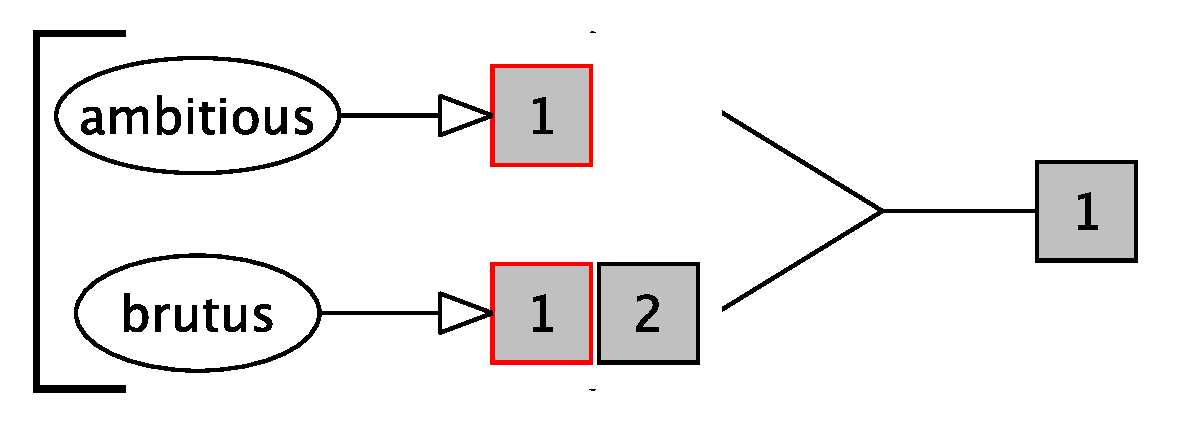
\includegraphics[scale=1]{pics/KWquery-processing}
}%
\caption{Processing of the keyword query ``brutus AND ambitious''. The only
document containing both terms is the document 1, from the
Table~\ref{tab:indexing}.}
\label{fig:KWquery}
\end{figure}

\subsection{Phrase Query Processing}

The position of terms in a document is very important, as it can change the
meaning of these terms in the document. For example the keyword query
``\emph{stanford AND university}'' may return a document containing the
sentence ``The inventor Stanford Ovshinsky never went to university''. However
the given query suggested to search information about a University in
Stanford. The returned document is then irrelevant to the query, to what really
is needed by the user. In order to perform more precise search, the position
information about the terms in documents is necessary. Indeed restricting the
search to documents having the keyword terms appear consecutively one after the
other will discard irrelevant documents. As four terms are between Stanford
and University in the former example, such a document will not be returned if
restricting to zero words in-between. The query that takes into account the
position of terms within documents are called \emph{Phrase queries}.

A \emph{n-gram} is a sub-sequence of n terms in the document. For instance, a
bi-gram (i.e., a sub-sequence of two terms) in document 1 in
Table~\ref{tab:indexing} can be ``I was'' or ``Brutus killed''. There exist
two ways to handle phrase queries. The first one relies on indexing n-gram
occurring in the collection. Indexing bi-gram would follow the same process as
in the Table~\ref{tab:indexing}, but with bi-gram instead of single terms.
However it restricts to bi-gram only, and to search for tri-gram (i.e., three
terms in the sub-sequence) it would mean to index also tri-gram. This is highly
inefficient as a huge storage space is then needed. The second way uses the
position information of terms within documents to process phrase queries. Thus
only uni-gram (i.e., one term in the sub-sequence) are indexed with the relative
position of each term. Also we can handle this way phrase queries with any
number of terms in the sub-sequence.

\subsubsection{Phrase queries processing algorithm}

The first step in processing phrase queries is the same as processing
keyword queries: after retrieving inverted lists of each term, we perform
operations on the inverted lists to get the list of documents identifiers
matching the terms in the query. The second step consists in filtering these
documents according to the position information. The algorithm to discard or
not a document works on the positions of keywords occurring in a same document,
and is as follows:
\begin{enumerate}
  \item[] Let R be the list of documents identifiers that results from the
  first step.
  \item For each document i in R.
  \item Retrieve the list $P_{T1,i}$ of positions for the term T1 in document i,
  and the list $P_{T2,i}$ of positions for the term T2 in document i.
  \item Compare position values $p_1 \in P_{T1,i}$ and $p_2 \in P_{T2,i}$
  \begin{enumerate}
    \item The absolute difference between $p_1$ and $p_2$ is \emph{greater than}
    1 $\Rightarrow$ within the list with the lower value, we advance until
    reading a position greater than the other value.
    \item The absolute difference between $p_1$ and $p_2$ is \emph{equal to} 1
    $\Rightarrow$ the current document is kept and we go to the next document
    in R.
  \end{enumerate}
\end{enumerate}
The Figure~\ref{fig:PQquery} depicts with dashed lines the comparisons performed
in the step 3 in the former algorithm. We first compare 1 and 8 and keep on
reading values in P1 until the value 20. Then the comparison between 20 and 8,
and so on. The algorithm stops at comparison 5, as the difference is equal to
1. The document is thus kept in the results of the phrase query. In the
Table~\ref{tab:indexing}, the phrase query ``brutus killed'' would match the
document 1, as the terms appear respectively in positions 7 and 8. We can note
that as the difference computed in steps 3 is absolute, the phrase query
``killed brutus'' also matches that document. This reflects the ``bag of
words'' query model in Information Retrieval.

\begin{figure}
\centering
\resizebox{0.9\linewidth}{!}{%
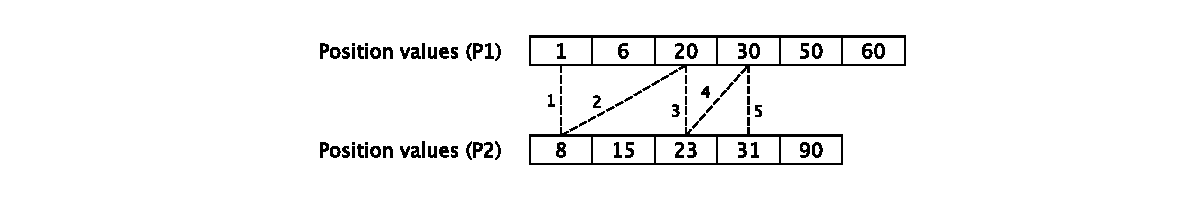
\includegraphics[scale=1]{pics/PQsearch}
}%
\caption{Documents filtering based on the position of terms. P1 and P2 are two
positions lists of two different terms occurring in the same document. Dashed
lines represent comparison between position values. The order in which these
comparisons are made is indicate by their label number.}
\label{fig:PQquery}
\end{figure}


\chapter{Semantic Web}{
The World Wide Web has drastically changed over the past decade. Tim
Berners-Lee is the person who introduced the idea of linked information thanks
to HyperText Markup Language (HTTP), which is the core of the web. The
expectations Tim Berners-Lee had of a global information space, where any data
can be read, written and shared is now concrete. The challenge is now to
organize this massive amount of knowledge and to improve the interactions
people have with this huge and complex system.

A major problem of the web comes directly from its core, the HTML. Thanks to
HTML, documents can be linked together, and a human can move from one document
to an other with those links. A computer is able to interpret this language,
however the content of documents is written in natural language, and is then
only accessible to people.

Most of the content on the web is only readable by people. One can read the
information of documents and understand its meaning. On the opposite, computers
only know to which documents a document is related to thanks to HTML markups.
However they do not carry descriptions about the content of a document and how
two documents are related to each other.

This is the reason why Internet applications like search engines have limited
capabilities. A search engine looks for a term T in a document, but it cannot
search for related documents, as it lacks a formal description of the content.
A search engine help people look for data, but in the end to find precise
information, he has to himself follow HTML links. This is a highly consuming
task, with limited results.

A solution is to provide computers with comprehensible Web data is to describe
documents and their relationships with meaningful metadata. The Semantic
Web aims to merge web resources with machine-understandable data to enable
people and computers to work in cooperation and to simplify the sharing and
handling of large quantities of information.

In this chapter I present the vision of the Semantic Web, before describing the
various technologies in the Semantic Web. Then I present how Web data is
represented to make it machine-understandable. Finally I present some projects
that use Semantic Web technologies.
}
%%%%%%%%%%%%%%%%%%%%%%%%%%%%%%%%%%%%%%%%%%%%%%%%%%%%%%%%%%%%%%%%%%%%%%%%%%%%%%
\label{chap:SW}
\section{The Framework}

The Semantic Web defines a set of technologies which are a standard on how to
describe, manipulate and query Semantic data to have in the end a solid base of
machine-readable knowledge. The Semantic Web presents a layer hierarchy
(Figure~\ref{fig:sw-stack}), where each layer has its own purpose. A layer of
this Semantic Web Stack uses the information provided by layers below. This
shows how Semantic Web is made possible and how it is not a replacement of the
current Web but an extension.

\begin{figure}
\centering
\resizebox{0.5\linewidth}{!}{%
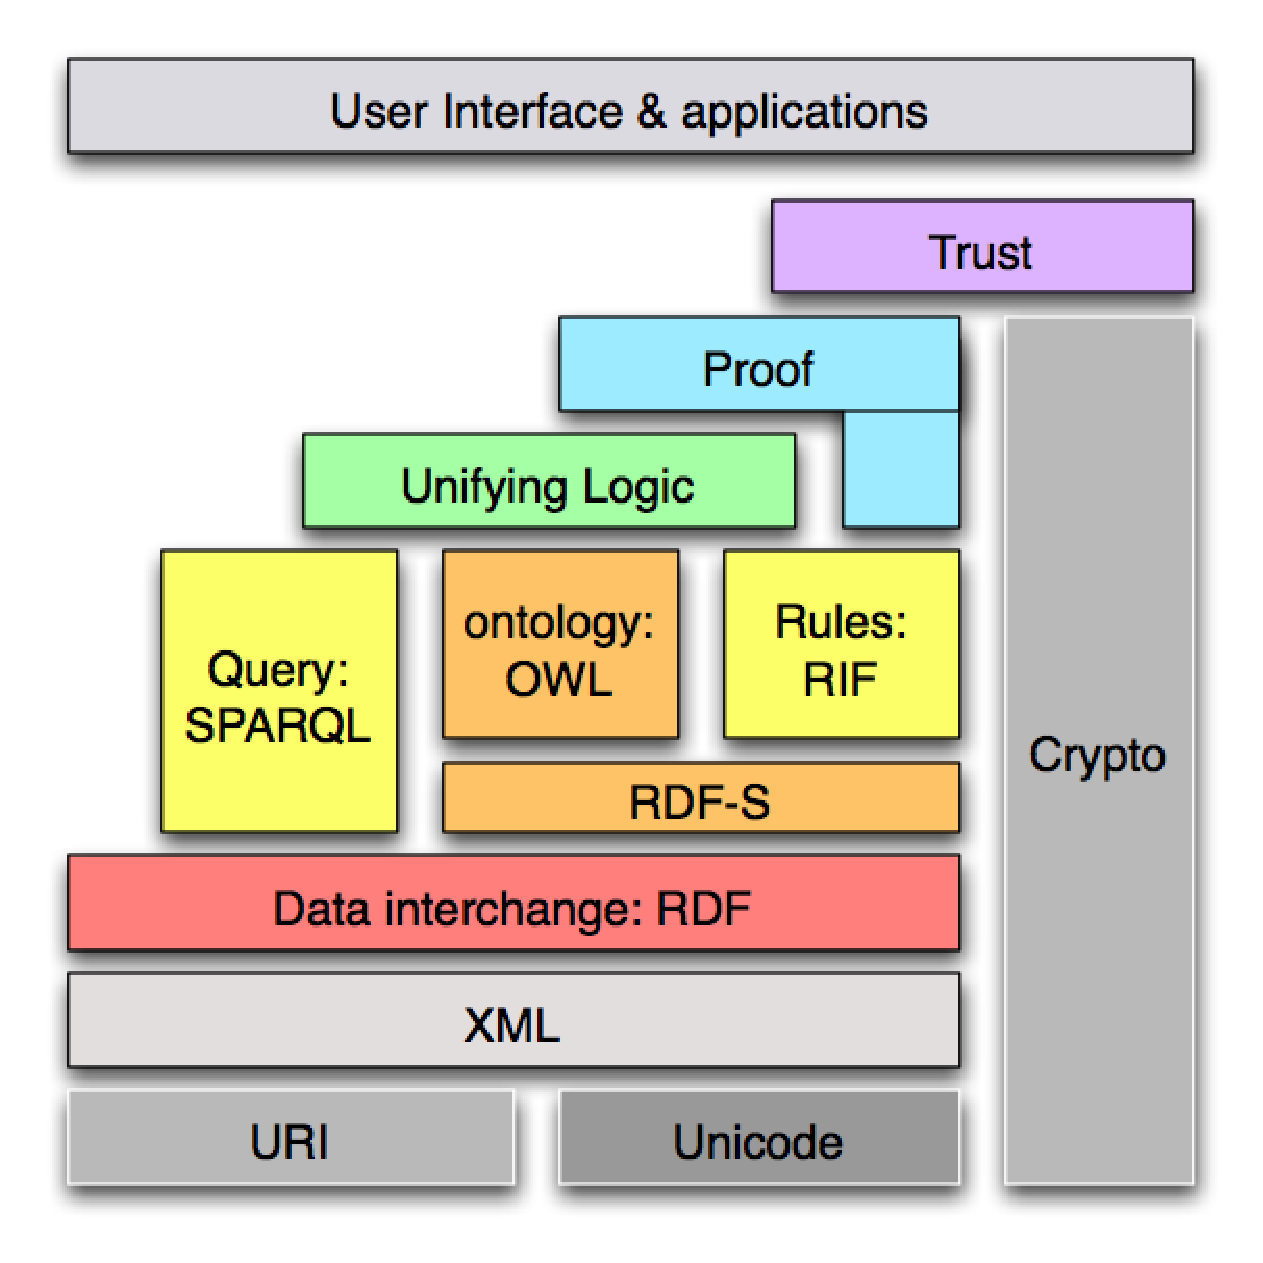
\includegraphics[scale=1]{pics/SemWebStack}
}%
\caption{The Semantic Web Stack. It presents each layer of the Semantic Web,
where each have a defined a purpose and that make the Semantic extension of the
Web as we know it possible.}
\label{fig:sw-stack}
\end{figure}

\begin{description}
\item[Uniform Resource Identifier (URI)] provides means for uniquely
identifying semantic web resources.
\item[Unicode\footnote{\url{http://www.unicode.org/standard/versions/}}] 
serves to represent and manipulate text in many languages. Semantic Web should
also help to bridge documents in different human languages, so it should be
able to represent them.
\item[XML] extensible Markup Language (XML) is the standard syntax that
enables creation of documents composed of structured data. Semantic web gives
meaning (semantics) to structured data. 
\item[Resource Description Framework (RDF)] is the standardized representation
of meta-data.
\item[RDF Schema (RDFS)] provides basic vocabulary for RDF.
\item[Web Ontology Language (OWL)] extends RDFS and allows a more complex
representation of resources (i.e., ontology). It gives then the possibility of
more advanced reasoning over data.
\item[SPARQL] is a RDF query language. It can be used to query any RDF-based
data and provide information to Semantic Web applications.
\item[Logic-Proof] a reasoning layer that infers new knowledge from the data.
\item[Trust] prove the trustfulness of the data thanks to cryptographic
techniques.
\item[User Interface] is the final layer that will enable humans to use
semantic web applications.
\end{description}

URI is a string that is used to identify resources over the Internet. It is
often used by markup languages to specify external documents or a specific
section of that document. For instance \emph{\url{http://di2.deri.ie/}} is an
URI that describes the Data Intensive Infrastructure unit.

An ontology in Information Science is a formal representation of knowledge as a
set of concepts within a domain, and the relationships between those concepts.
It is used to reason about the entities within that domain, and may be used to
describe the domain. For example we can have a simple ontology describing
animals like rats and cats are mammals; a mammal is an animal. Such an ontology
can be used when searching for terms in different domains.

\section{RDF: Resource Description Framework}

RDF is a framework that allows data on the web to be shared and reused across
applications. It provides features that facilitate data to be interchange
between datasets, even if they have different ontology.
RDF is used to describes things in the Internet, and the relations between
things. It extends the linking structure of the Web to use URIs to name the
relationship between concepts or objects as well as the two ends of the link.
This linking structure of the Web forms a directed, labeled graph called
\emph{RDF graph}, where the edges represent the relationship between two
objects, the graph nodes.

\subsection{RDF Model}

RDF is a standard
model\footnote{\url{http://www.w3.org/TR/2004/REC-rdf-concepts-20040210/\#section-Concepts}}
for data interchange on the Web. Two connected nodes and the named relation
form a \emph{triple}. The set of triples form the RDF graph. The three parts
that compose a triple are:
\begin{enumerate}
  \item a \emph{subject}: the resource that this triple describes.
  \item an \emph{object}: the resource that the subject is related to.
  \item a \emph{predicate}: the description of the link between the subject and
  the object.
\end{enumerate}
The Figure~\ref{fig:rdf-triple} depicts a triple as a node-arc-node
link. The direction of the arc is significant: it always points toward the
object. The nodes of an RDF graph are its subjects and objects. The meaning
given to a RDF graph is the conjunction of all its triples.

A RDF graph defines three types of nodes:
\begin{description}
\item[Literal] a literal is a simple string, used to describe dates, titles or
any text in natural language. A literal may be \emph{plain} or \emph{typed}:
	\begin{itemize}
	  \item A plain literal is a string combined with an optional language tag.
	  \item A typed literal is a string combined with a datatype URI.
	\end{itemize}
\item[URI reference (URIref)] a URIref is a Unicode string used in a RDF graph
to represent URIs, and it can have an optional fragment identifier which is
indicated by the character ``\#''. For example the URI reference
\url{http://www.w3.org/2000/01/rdf-schema#comment} shows the URI before \#, and
the fragment ``comment'' that indicates which identifier to use within the URI.
This particular fragment ``comment'' is used to describe the subject resource.
\item[Blank Node] a blank node refers to resources that are not identified.
\end{description}
In a triple, the subject can be either a URIref or a blank node. The predicate
must be a URIref, while the object can be either one of the three node types.

The URI tends to be very long, which becomes inconvenient when using frequently
a same URIref. QName is a name space used as an abbreviation of a URIref. Its
syntax is \emph{URI:fragment}. For example the fragment ``comment'' within the
URI \url{http://www.w3.org/2000/01/rdf-schema#} can be shortened to
\emph{rdfs:comment}, where rdfs is mapped to the URI.

In the drawing convention of a RDF graph, URIrefs and blank nodes are drawn with an
ellipse, and literals with a rectangle. The Figure~\ref{fig:rdf-graph} depicts
a RDF graph describing the work ``The Lord of the Rings'' written by J.R.R
Tolkien. In this graph, the QNames ``dbpprop'' and ``dbpedia-owl'' map
respectively to \emph{\url{http://dbpedia.org/property/}} and
\emph{\url{http://dbpedia.org/ontology/}}. This graph provides three different
triples describing the sequel. The RDF graph gives the meaning that the
resource \url{http://dbpedia.org/page/The_Lord_of_the_Rings} has for author
J.R.R Tolkien, that it was released in the years 1954-55 and that a portion of
the English abstract is ``The Lord of the Rings is an epic\ldots''. We also
know that an unknown resource preceding ``The Lord of the Rings" novel was also
written by Tolkien.

\begin{figure}
\resizebox{\linewidth}{!}{%
\subfloat[A triple]{%
\centering
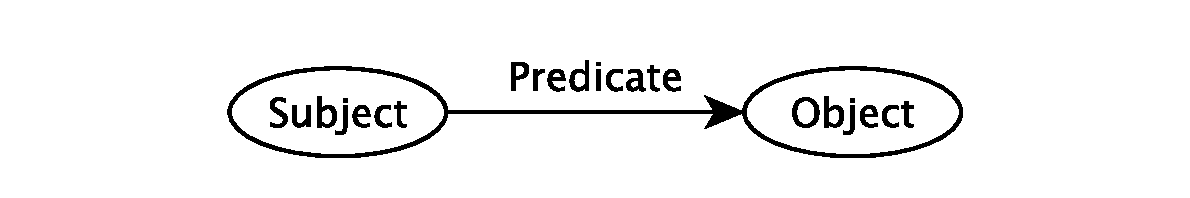
\includegraphics[scale=0.4]{pics/rdf-triple}
\label{fig:rdf-triple}
}\quad
\subfloat[A RDF graph describing the work ``The Lord of the Ring'' by J.R.R
Tolkien, using several QNames.]{%
\centering
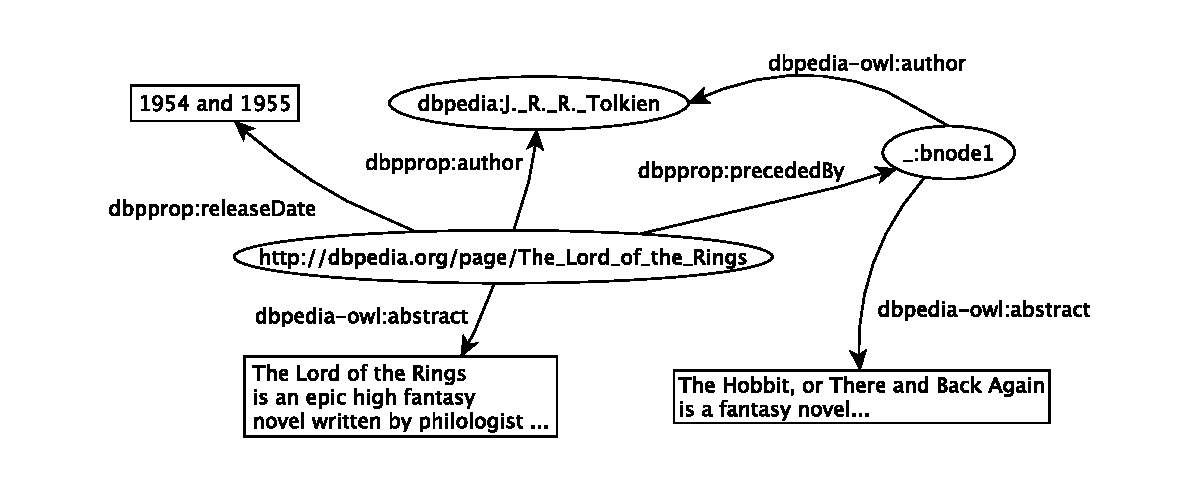
\includegraphics[scale=0.5]{pics/rdf-graph}
\label{fig:rdf-graph}
}}%
\caption{The RDF model used to represent knowledge.}
\end{figure}

\subsection{RDF Serialization}

Many serialization format for RDF have been developed, such as
RDFa\footnote{\url{http://www.w3.org/TR/xhtml-rdfa-primer/}} which is used to
embed RDF triples within XML documents. However during my internship only the
serialization format
\emph{N-Triple}\footnote{\url{http://www.w3.org/TR/rdf-testcases/\#ntriples}}
has been actively used, and so it will be the only one described here. Using
the N-Triple format, the triples within a RDF graph can be serialized with a
line-based plain text format. It is a format recommended to interchange data
between different applications.

This serialization uses an Extended Backus-Naur Form grammar, where each triple
is written into a line, ending with a point. The format is {\bfseries
\emph{Subject Predicate Object .}}\hs.
A URIref is written enclosed between the characters \emph{'$<$' '$>$'}. The
literals are written between double quotes, followed by an optional language
tag \emph{@language} for plain literals (e.g. ``bird"@en), and by
\emph{'\^{}\^{}'URIref} for typed literal (e.g.
``abc"\^{}\^{}$<$\url{http://example.org/datatype1}$>$, where abc is of type
datatype1). A blank node is represented by \emph{'\_':name}, where name is an
internal identifier which allows to have several blank nodes within a RDF
graph. The RDF graph in the Figure~\ref{fig:rdf-graph} can be serialized in
N-Triples format as in Table~\ref{tab:TL-ntriples} where \emph{TLR} refers to
the URI \url{http://dbpedia.org/page/The_Lord_of_the_Rings}.

\begin{table}
\centering
\resizebox{0.9\linewidth}{!}{%
\begin{tabular}{lclclcl}
$<$TLR$>$&\phantom{a}&$<$dbpprop:author$>$&\phantom{a}&$<$dbpedia:J.\_R.\_R.\_Tolkien$>$
&\phantom{a}&.\\
$<$TLR$>$&\phantom{a}&$<$dbpprop:releaseDate$>$&\phantom{a}&``1954 and
1955''&\phantom{a}&.\\
$<$TLR$>$&\phantom{a}&$<$dbpedia-owl:abstract$>$&\phantom{a}&``The Lord of
the Rings is an epic\ldots''&\phantom{a}&.\\
$<$TLR$>$&\phantom{a}&$<$dbpprop:precededBy$>$&\phantom{a}&$\_:bnode1$&\phantom{a}&.\\
$\_:bnode1$&\phantom{a}&$<$dbpedia-owl:author$>$&\phantom{a}&$<$dbpedia:J.\_R.\_R.\_Tolkien$>$&\phantom{a}&.\\
$\_:bnode1$&\phantom{a}&$<$dbpedia-owl:abstract$>$&\phantom{a}&''The Hobbit, or
There and Back Again is a fantasy novel\ldots''&\phantom{a}&.\\
\end{tabular}
}%
\caption{N-Triple representation of the RDF graph in
Figure~\ref{fig:rdf-graph}.}
\label{tab:TL-ntriples}
\end{table}

\subsection{SPARQL}

The RDF model introduce a mean to represent data and any type of data can,
at least to some degree, be represented in this model. SPARQL\footnote{SPARQL:
\url{http://www.w3.org/TR/rdf-sparql-query/}} is a standardized query language
for RDF. Designed so that queries can be expressed across diverse data, SPARQL
is able to express not only conjunction and disjunction of RDF graphs but also
complex queries, e.g. by using supplementary binary operators such as
arithmetic operators and comparisons in various filters.

A SPARQL query contains a set of \emph{triple patterns} that matches a
sub-graph of RDF graphs. Triple patterns are expressed in the same way as RDF
triples, i.e., subject, predicate, object, the difference being that any part of
that triple can be a variable. Typical SPARQL queries are graph patterns
combining SQL-like logical conditions over RDF statements with
regular-expression patterns. The result of a query is a set of sub-graphs
matching precisely the graph pattern defined in the query. For instance, the
SPARQL query
\begin{quote}
\begin{flushleft}
PREFIX dbpprop:    $<$http://dbpedia.org/property/$>$\\
SELECT ?abstract\\
WHERE\\
\{\\
\begin{quote}
$<$TLR$> \; <$dbpprop:author$> \;$ ?abstract $\;$ . 
\end{quote}
\}
\end{flushleft}
\end{quote}
has a single triple pattern that matches the first row of the triples in the
Table~\ref{tab:TL-ntriples}. The first line shows the QName used in the query.

% \subsection{Reasoning}
% 
% Reasoning is the cognitive process to look for conclusions and beliefs.
% Reasoning allows to create links between two objects that are somehow related
% but only implicity, granting thus the machine to enlarge its searching scope.
% For example, we know that a monkey is a mamal and that mammals are an animal
% species, but how can a machine deduces that a monkey is also an animal. Through
% reasoning over RDF graphs, it is possible to ``create'' more knowledge,
% \emph{implicit} knowledge, from the explicit relations already existing. For
% example, the RDFS schema possesses inheritance reasoning capabilities
% through the property \emph{subClassOf} such as
% \begin{quotation}
% (rdf:type Morris Cat)
% 
% (rdfs:subClassOf Cat Mammal),
% \end{quotation}
% which implies that Morris is also a sub-class of mammal.


%%%%%%%%%%%%%%%%%%%%%%%%%%%%%%%%%%%%%%%%%%%%%%%%%%%%%%%%%%%%%%%%%%%%%%%%%%%%%%
\chapter{SIREn}{
People are using more and more Semantic Web technologies and the quantity of
Semantic data will keep on expanding. Scalable and performant RDF management
systems are then becoming a necessity for semantic applications in order to use
thoroughly semantic data. Moreover traditional search engines do not use the
structured information available with semantic data. Taking the e-commerce as
an example, looking for a particular product is done by entering keyword
queries into the search engine and web pages are returned. However these
documents are most of the time irrelevant as they only include the key words,
but are not necessarily about the product itself. Also such web pages are
likely to provide information about other unrelated products as well. What is
really looked for then is the \emph{entity} of the product and anything that
can be related to that entity.

Sindice\footnote{Sindice: \url{http://sindice.com/}} is a web service which
purpose is to offer efficient searching capabilities over the semantic data.
Sindice is built on top of the Semantic Information Retrieval Engine,
SIREn\footnote{SIREn: \url{http://siren.sindice.com/}}, a system based on
Information Retrieval which goal is to search not for web pages but for
``entities''.

In this chapter, the indexing model of SIREn is presented before introducing
its query model.}
%%%%%%%%%%%%%%%%%%%%%%%%%%%%%%%%%%%%%%%%%%%%%%%%%%%%%%%%%%%%%%%%%%%%%%%%%%%%%%
\label{chap:BG-siren}
\section{Related Work}

In this section, we describe the current approaches for indexing RDF data,
before reviewing the existing search models for (semi) structured data.

\subsection{Retrieval of RDF Data}

The growth of RDF data incurs the need of efficient and scalable data
management systems. Several systems have been proposed based on Relational
DataBases Management Systems (RDBMS)~\cite{beckett:2003:swss-rdbms}. RDF data
management systems are able to store a large amount of data and use SPARQL as a
query language which allows to perform complex searches over the collection. A
user is able to perform complex request when the database schema is known.
However given the heterogeneous data collection on the web, the added value of
SPARQL is limited. Indeed it is difficult to write precise queries since the
data structure and the ontology may vary from one dataset to an other.

Other
approaches~\cite{guha:2003:tap,ding:2005:swoogle,harth:2008:swse,cheng:2008:falcons}
carried over keyword-based search to Semantic Web and RDF data in order to
provide ranked retrieval using content-based relevance estimation. In
addition, such systems are easier to scale due to the simplicity of their
indexing scheme. However, such systems are restricted to keyword search and do
not support structural constraints. These systems do not consider the rich
structure provided by RDF data.

A first step towards a more powerful search
interface combining imprecise keyword search with precise structural
constraints has been investigated by Semplore~\cite{wang:2009:semplore}.
Semplore has extended inverted index to encode RDF
graph approximations and to support keyword-based tree-shaped queries over RDF
graphs. However the increase of query capabilities comes at a cost, and the
scalability of the system becomes limited.

\subsection{Search Models for (semi) Structured Data}

In addition to standardised query languages such as SPARQL, a
large number of search models for semi-structured data have been developed. Some
of them focus on searching structured
databases~\cite{agrawal:2002:dbxplorer,bhalotia:2002:banks,hristidis:2002:discover,liu:2006:sigmod},
XML documents~\cite{cohen:2003:xsearch,guo:2003:xrank,liu:2007:xseek} or
graph-based data~\cite{abiteboul:1996:lorel,kachiola:2005:vldb,li:2008:ease}
using simple keyword search. Simple keyword-based search has the advantages of
\begin{inparaenum}[(1)]
\item being easy to use by users since it hides from the user any structural
information of the underlying data collection, and
\item of being applicable on any scenarios. 
\end{inparaenum}
On the other hand, the keyword-based approach suffers from limited capability
of expressing various degrees of structure when users have a partial knowledge
about the data structure.

Other
works~\cite{kasneci:2008:naga,mandreoli:2009:edbt,wang:2009:semplore,dong:2007:sigmod,fletcher:2009:theory-search}
have extended simple keyword-based search with structured queries
capabilities. \cite{dong:2007:sigmod,fletcher:2009:theory-search} propose a
partial solution to the lack of expressiveness of the keyword-based approach
by allowing search using conditions on attributes and values.
\cite{kasneci:2008:naga,mandreoli:2009:edbt,wang:2009:semplore} present more
powerful query language by adopting a graph-based model. However, the increase
of query expressiveness is tied with the processing complexity, and the
graph-based models
\cite{kasneci:2008:naga,mandreoli:2009:edbt,wang:2009:semplore} are not
applicable on a very large scale.

The search model introduced in Section~\ref{sec:siren-model} is similar to
\cite{dong:2007:sigmod,fletcher:2009:theory-search}, i.e., it is defined
around the concept of attribute-value pairs. However, our model is more
expressive since it differentiates between single and multi-valued attributes
and it considers the provenance of the information.

\section{Formal Model}
\label{sec:siren-model}

The expansion of Semantic Web applications has increased considerably and it
will continue on this progression. A wide range of different technologies has
been developed to represent and use semantic data. For the purpose of covering
a majority of data sources when searching for entities, a formal model has been
introduced. In this section, I give a summary of a labeled directed graph
model, before describing its query model.

\subsection{Entity Attribute-Value Model}

Semantic data can be used to describe any kind of data, from a physical person
to an abstract notion. These \emph{entities} are at the core of any data and
are the unit that is to be searched for with SIREn. This section presents
fundamentals about the Entity Attribute-Value model, a generic model which goal
is to support scenarios involving entities.

A Semantic graph (e.g. a RDF graph) is a graph that gives information about
several entities somehow related to each other. This graph can then be split
into sub-graphs, each one describing a particular entity. A \emph{star graph},
i.e., an entity at the center with associated incoming and outgoing relations.
For instance, the RDF graph in Figure~\ref{fig:rdf-graph} can be split into
three entities, as depicted in the Figure~\ref{fig:entities}. The graph
describing ``The Lord of the Rings'' work is divided into the
\emph{\url{http://dbpedia.org/page/The_Lord_of_the_Rings}}, \emph{\_:bnode1}
and \emph{dbpedia:J.\_R.\_R.\_Tolkien} entities.
% Also, the FOAF file from the
% Listing~\ref{lst:foaf} can be splitted into three entities: \emph{Giovanni
% Tummarello}, \emph{Renaud Delbru} and \emph{Stephane Campinas}.
The star graph gives information about the entity and is then generically
called an \emph{entity description}.

A \emph{dataset} is a source of semantic data, such as a domain or a site web
and it gives the \emph{context} of the data it contains. An \emph{attribute}
refers to the relation between an entity and an object, e.g. the predicate in
a RDF triple. For example ``dbpedia-owl:author'', ``dbpedia-owl:abstract'' and
``dbpprop:precededBy'' are the attributes associated with the \_:bnode1
entity. An attribute can also be \emph{multi-valued} as a book can have
multiple authors for instance. A \emph{value} refers to the node related to an
entity.

\begin{figure}
\centering
\resizebox{\linewidth}{!}{%
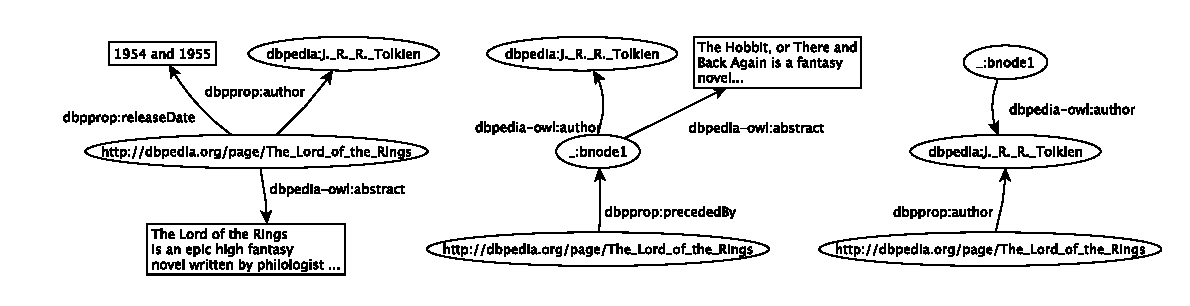
\includegraphics[scale=1]{pics/entities}
}%
\caption{A representation of the RDF graph in Figure~\ref{fig:rdf-graph}
divided into three entities: \emph{The Lord of the Rings}, \emph{\_:bnode1}
and \emph{Tolkien}.}
\label{fig:entities}
\end{figure}

\subsubsection{Node-Labelled Tree Model for RDF}

SIREn uses a node-labelled tree structure to capture the relationship between
values, attributes, entities and datasets. Taking the RDF data model (the
triple) as a support, the tree represent four kinds of nodes as depicted in the
Figure~\ref{fig:tree-model}:
\begin{itemize}
  \item the \emph{dataset} that indicates the context of the data.
  \item the \emph{entity} (the subject).
  \item the \emph{attribute} (the predicate).
  \item the \emph{value} (the object).
\end{itemize}
Each node can refer to one or more terms. In the case of RDF, a term is not
necessarily a word from a literal, but can be an URI or a local blank node
identifier.

A node-labelled tree model enables to encode and efficiently establish
relationships between the nodes of a tree. The two main types of relations are
Parent-Child and Ancestor-Descendant. To support these relations, the
requirement is to assign \emph{unique identifiers}, called node labels, that
encode the relationships between the nodes. The Dewey
encoding~\cite{beyer:2002:ordered-xml} is a simple node labelling scheme. In
Dewey Order encoding, each node is assigned a vector that represents the path
from the tree’s root to the node and each component of the path represents the
local order of an ancestor node. Using this labelling scheme, structural
relationships between elements can be determined efficiently. An element u is
an ancestor of an element v if label(u) is a prefix of label(v). The
Figure~\ref{fig:dewey-encoding} depicts the tree representation of the RDF
graph in Figure~\ref{fig:rdf-graph} using the Dewey encoding. The dataset is
the domain of the URI the graph is hosted at. In that representation, the
qualified names (i.e., QNames) have been removed in order to keep only the
property name, for clarity purpose since the property has the same semantic
even if the QNames are different (e.g., dbpprop:author and dbpedia-owl:author).
For example the entity ``The\_Lord\_of\_the\_Rings'' with vector [1.1], we can
find that it is a parent of the value node ``J.R.R.\_Tolkien'' with vector is
[1.1.2.1].

\begin{figure}
\centering
\subfloat[Conceptual representation of the node-labelled tree model.]{
\resizebox{0.34\linewidth}{!}{%
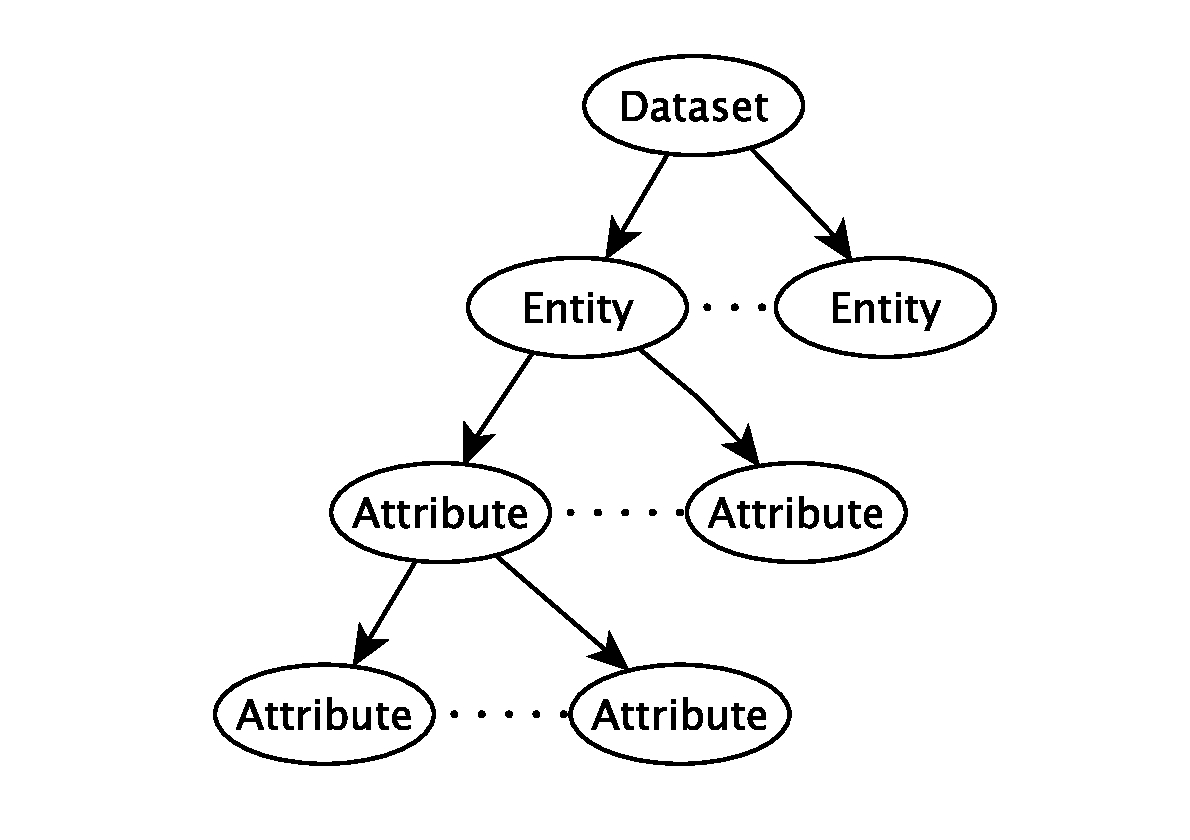
\includegraphics[scale=1]{pics/tree-model}
\label{fig:tree-model}
}}\quad
\subfloat[Node-labelled tree model with Dewey encoding of the dataset in
Figure~\ref{fig:rdf-graph}.]{
\resizebox{0.6\linewidth}{!}{%
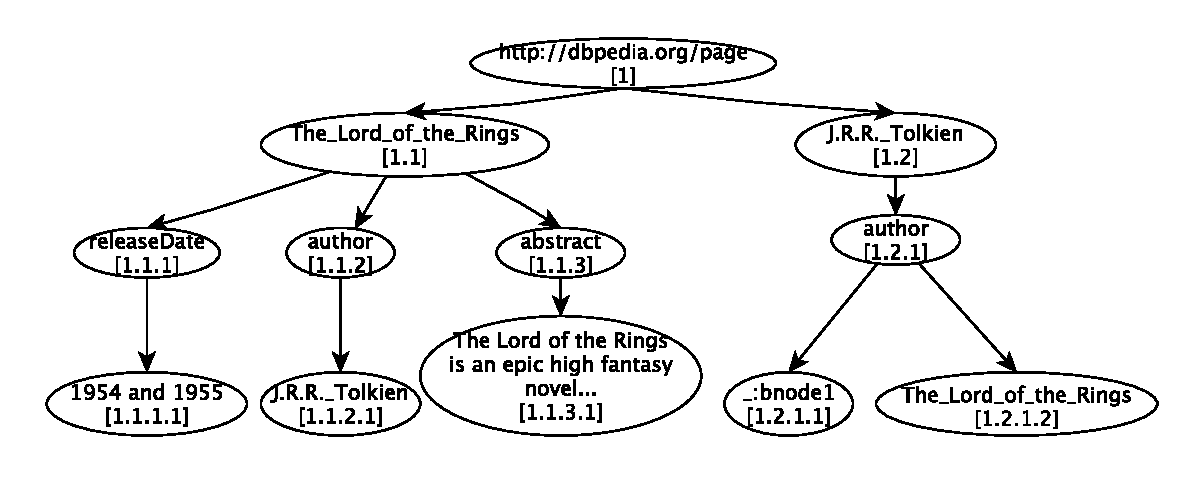
\includegraphics[scale=1]{pics/dewey-encoding}
\label{fig:dewey-encoding}
}}
\caption{The node-labelled tree model.}
\end{figure}

\subsection{Query Model}
\label{sec:siren-query-model}

Entities present a semi-structured structural view, and not a ``bag of
words'' as in traditional search engines. Therefore the query model search
entities with Boolean combinations of attribute-value pairs.

SIREn supports three different types of queries:
\begin{description}
\item[full-text:] traditional keyword query, useful when the schema of the
dataset is unknown;
\item[structural:] complex queries specified in a star-shaped structure, useful
when the data schema is known;
\item[semi-structural:] a combination of the two where full-text search can be
used on any part of the star-shaped query, useful when the data structure is partially known.
\end{description}
These query types provide different level of complexity, depending on the
knowledge of the data structure by the user. But the SIREn engine is aimed to
be used by other machines, and the possibility of complex queries are then
needed. The Figure~\ref{fig:star-query} depicts a star-shaped query that
matches the ``The Lord of the Rings'' entity from the
Figure~\ref{fig:entities}. This semi-structural query makes use of full-text
search through the use of keywords (e.g. ``tolkien'' or ``lord''). We can also
embedded Boolean search inside nodes, then the matching of entities having the
keywords ``lord'' and ``rings'' are marked as a positive match for the value
of an abstract (or label) attribute. The wildcard can also be used to describe
unknown relations between nodes. This search model is developed to find
entities that best match an entity description pattern (e.g. star-shaped
pattern).

In opposite to the full-text logical view where words are seen are seen as a
single bag of words, in the semi-structured view, the words are assigned to
multiple distinct bag of words, one for each value and attribute. Consequently,
it is possible to distinguish when words occur in a same value or different
values and avoid false-positive answers.

\begin{figure}
\centering
\resizebox{0.5\linewidth}{!}{%
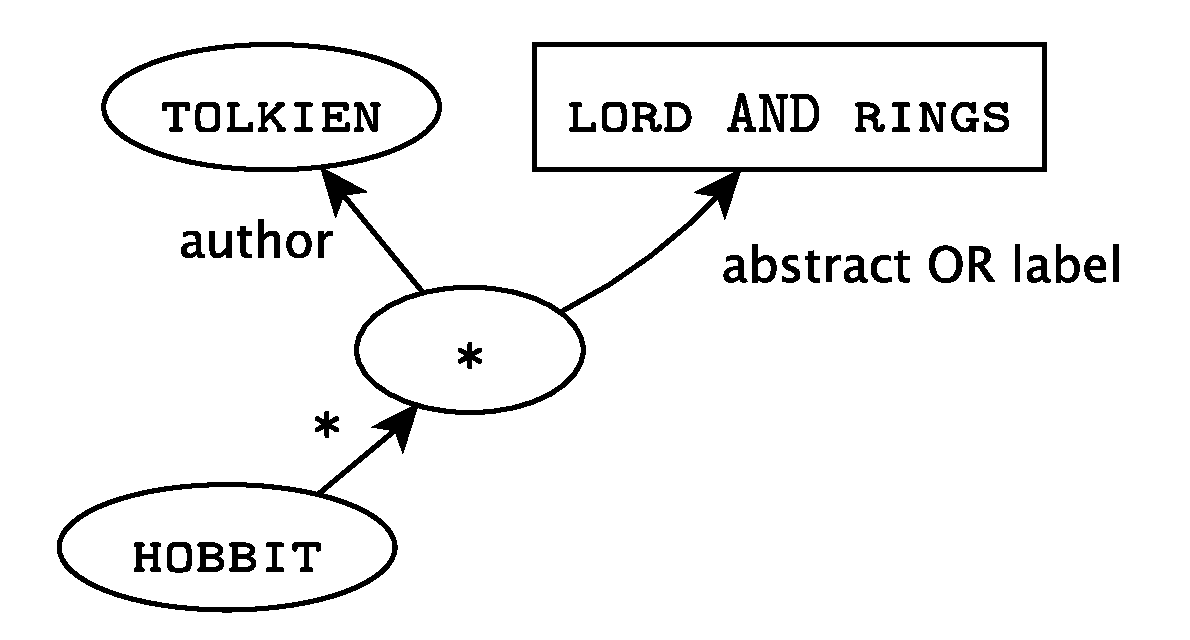
\includegraphics[scale=1]{pics/query}
}%
\caption{A star-shaped query matching the entity ``The Lord of the Rings''
from the Figure~\ref{fig:entities}. The character * stands for the wildcard
variable.}
\label{fig:star-query}
\end{figure}

\section{Model Implementation}

This section aims to present the implementation of the Entity Attribute-Value
model and of the query model over an inverted index. An overview of the
inverted index construction is presented with the entity-centric indexing
before describing more thoroughly the indexing structure.

\subsection{Entity-Centric Indexing}
\label{sec:ent-cent-indexing}

The search unit of the SIREn engine is an entity. As such,
SIREn aims to index entities (i.e., star graphs), and not documents
as the Section~\ref{sec:IR-indexing} presents it.
With a \emph{document-centric} indexing, every terms belong to a same document.
For instance the RDF graph in Figure~\ref{fig:rdf-graph} can be
taken as a whole document, since all data has been taken from the same web page
\url{http://dbpedia.org/page/The_Lord_of_the_Rings}. However when searching for
the entity \emph{The Lord of the Rings}, we just want information about this
entity and not also about any related work. This is a reason why SIREn uses an
\emph{entity-centric} indexing.

With a document-centric indexing, all the terms from the N-Triples of the
Figure~\ref{fig:rdf-graph} are seen as one document.
Then any queries on one of those terms will return that document. With an
entity-centric approach, we index the three different entities separately as
reported in the Table~\ref{tab:TLR-ent-cent}.

\begin{table}
\centering
\resizebox{\linewidth}{!}{%
\begin{tabular}{lc@{\hs}llll}
\toprule
Entity &\phantom{a}& \multicolumn{4}{c}{N-Triples}\\
\cmidrule{3-6}
% \multicolumn{6}{c}{\phantom{a}}\\
{\bfseries TLR} & \multicolumn{5}{c}{\phantom{a}} \\
\multirow{3}{*}{\phantom{a}}&\multirow{3}{*}{\phantom{a}}&
$<$TLR$>$&$<$dbpprop:author$>$&$<$dbpedia:J.\_R.\_R.\_Tolkien$>$&$.$\\
&&$<$TLR$>$&$<$dbpprop:releaseDate$>$&``1954 and 1955''&$.$\\
&&$<$TLR$>$&$<$dbpedia-owl:abstract$>$&``The Lord of the Rings is an
epic\ldots''&$.$\\

{\bfseries \_:bnode1} & \multicolumn{5}{c}{\phantom{a}} \\
\multirow{3}{*}{\phantom{a}}&\multirow{3}{*}{\phantom{a}}&
$<$TLR$>$&$<$dbpprop:precededBy$>$&\_:bnode1&$.$\\
&&\_:bnode1&$<$dbpedia-owl:author$>$&$<$dbpedia:J.\_R.\_R.\_Tolkien$>$&.\\
&&\_:bnode1 &$<$dbpedia-owl:abstract$>$&''The Hobbit, or There and Back
Again is a fantasy novel\ldots''&$.$\\

{\bfseries dbpedia:J.\_R.\_R.\_Tolkien} & \multicolumn{5}{c}{\phantom{a}} \\
\multirow{2}{*}{\phantom{a}}&\multirow{2}{*}{\phantom{a}}&
\_:bnode1&$<$dbpedia-owl:author$>$&$<$dbpedia:J.\_R.\_R.\_Tolkien$>$&.\\
&&$<$TLR$>$&$<$dbpprop:author$>$&$<$dbpedia:J.\_R.\_R.\_Tolkien$>$&.\\

\bottomrule
\end{tabular}
}%
\caption{Entity-centric indexing on ``The Lord of the Rings'' RDF graph of
Figure~\ref{fig:rdf-graph}. Each entity is reported with its star graph in the
N-Triples format.}
\label{tab:TLR-ent-cent}
\end{table}

SIREn stores triples documents into a table where each
documents are stored as rows, a column having a meaning for the
document (e.g. title, abstract, \ldots). The Table~\ref{tab:doc-centric}
reports a document-centric strategy for semantic data like RDF triples, where
the first column stores the triple's subject, the second one the predicate and
the third one the object. As an attribute can be multi-valued, a lot of space is
wasted as three rows are used to store three triples where only the object
changes. In order to save space, thus improving indexing and querying
performances since less data to be written and read, SIREn uses a
representation format called \emph{N-Tuples}. It consists to collapse all
triples with a same predicate into one row and to remove the subject cell, as
depicted in the Table~\ref{tab:ent-centric}.

\begin{table}
\centering
\resizebox{0.8\linewidth}{!}{%
\subfloat[Document-centric indexing.]{%
\begin{tabular}{ccc}
\toprule
$<$ s $>$ & $<$ p1 $>$ & $<$ o1 $>\;.$ \\
$<$ s $>$ & $<$ p1 $>$ & $<$ o2 $>\;.$ \\
$<$ s $>$ & $<$ p1 $>$ & $<$ o3 $>\;.$ \\
$<$ s $>$ & $<$ p2 $>$ & $<$ o4 $>\;.$ \\
\bottomrule
\end{tabular}
\label{tab:doc-centric}
}\quad%
\subfloat[Entity-centric indexing.]{%
\begin{tabular}{cccc}
\toprule
$<$ p1 $>$ & $<$ o1 $>$ & $<$ o2 $>$ &$<$ o3 $>\;.$ \\
$<$ p2 $>$ & $<$ o4 $>$ & $\;.$ & \\
\bottomrule
\end{tabular}
\label{tab:ent-centric}
}}
\caption{Two different indexing strategies for semantic data, e.g. RDF triples.
The characters ``s'', ``p'' and ``o'' refer respectively to the subject,
predicate and object in a triple.}
\end{table}

\subsection{Inverted Index Structure}
\label{sec:siren-inv-lists}

Traditionally in Information Retrieval-based search engines, there are three
streams of integers that form an inverted list. A stream of documents
identifiers, a stream of term frequencies and a stream of positions.
In SIREn there are five stream of integers, being streams of entity
identifiers, of term frequencies, of attributes identifiers, of values
identifiers and of positions, identifiers taken from the Dewey encoding
depicted in the Figure~\ref{fig:dewey-encoding}. The term frequency corresponds
to the number of the term's occurrences in an entity description (e.g. a star
graph). The term position corresponds to the relative position of the term
within its node.

Because of the Dewey encoding, the identifiers numerical values have a
clustering effect: the entity identifier is local to a dataset, and the
attribute identifier is local to that entity, and so on. The
Figure~\ref{fig:siren-inv-lists} depicts the five stream of identifiers that
together form the inverted list in SIREn.
As an example for the locality of identifiers values, the position 5 and 7 in
the entity 10 (i.e., blue squares) describe a same term in a same value node
(i.e., value node with identifier 3). However the green square is local to the
same attribute 5, but not to the same value node.

The repetitive structure of semantic data (e.g. a same URI in the predicate
cell) implies that combining the entity-centric indexing with a delta encoding
of the inverted lists result in a compact inverted index structure. Indeed
because of the locality of the values, the gap between integers will be small.

\begin{figure}
\centering
\resizebox{0.32\linewidth}{!}{%
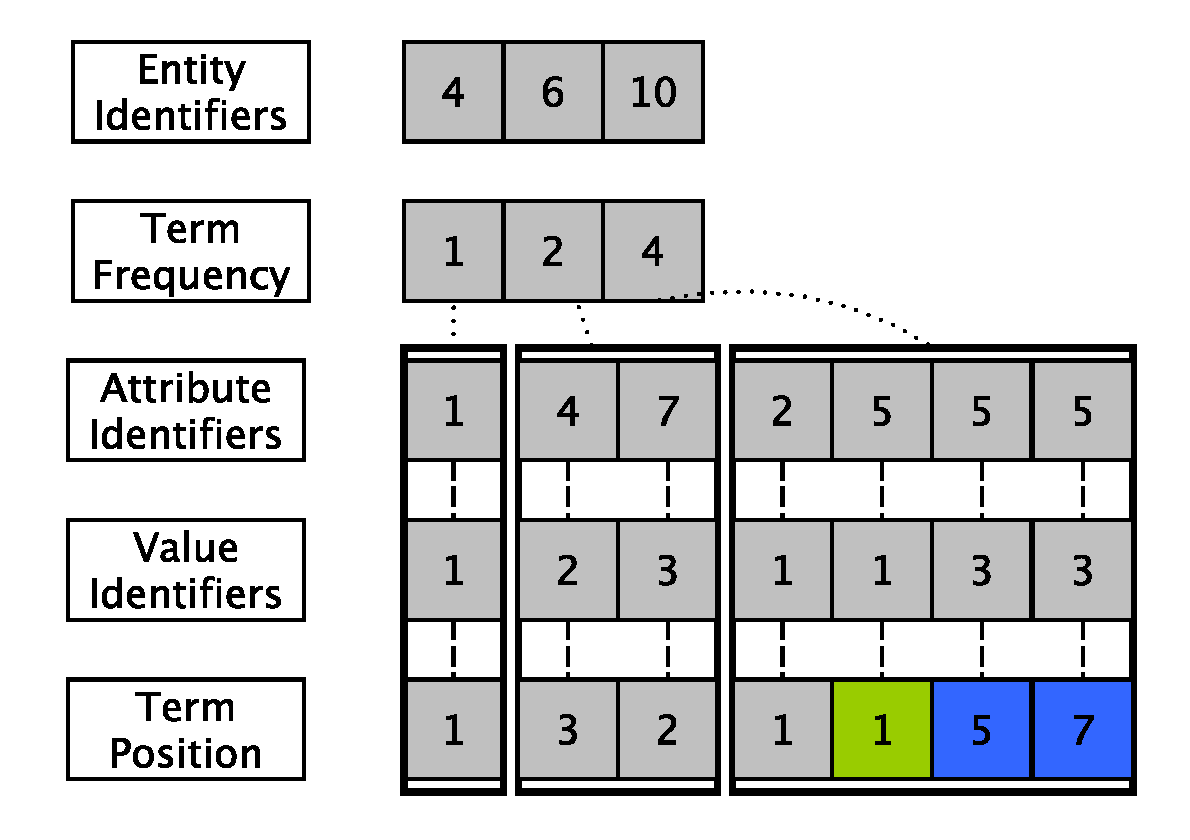
\includegraphics[scale=1]{pics/inverted-list-ex}
}%
\caption{Inverted Lists with the SIREn model.}
\label{fig:siren-inv-lists}
\end{figure}



%%%%%%%%%%%%%%%%%%%%%%%%%%%%%%%%%%%%%%%%%%%%%%%%%%%%%%%%%%%%%%%%%%%%%%%%%%%%%%
\chapter{Inverted List Compression}{
The inverted lists data, which are needed to process queries, are stored on
disk. This is the reason why reading the data is very costly on the queries
performance. The more data has to be read, and the slower the query response
will be. Thus inverted lists are compressed in order to reduce the number of
bytes read at query time, apart from the obvious goal to reduce disk space
consuming.

In this chapter, I present a state of the art of compression algorithms. While
Variable Byte is an algorithm that works on one integer at a time, Rice,
Simple family algorithms and Frame Of Reference-based techniques are
block-based. Given a block of integers from the list to compress, they aim to
compress it as best as possible using different approaches.}
%%%%%%%%%%%%%%%%%%%%%%%%%%%%%%%%%%%%%%%%%%%%%%%%%%%%%%%%%%%%%%%%%%%%%%%%%%%%%%
\label{chap:compression:state-of-the-art}
\section{Variable Byte}

Variable Byte (VByte) is an easy to implement algorithm, which makes it a
commonly used compression algorithm. VByte is a byte-aligned, i.e compression
at the byte level, algorithm that compress lists of values one integer at a
time. A compressed byte is divided in two parts
\begin{enumerate}
  \item the most significant bit is a \emph{flag} bit.
  \item the 7 bits left are used to store the integer.
\end{enumerate}
For an integer v to be compressed, the lower 7 bits are stored in one byte. The
flag is put at
\begin{inparaenum}[(a)]
\item 1 if there is still bits remaining in v or 
\item 0 otherwise.
\end{inparaenum}
This process is repeated until no more bits are left. The Table~\ref{tab:vbyte}
reports the algorithms used for VByte. The Algorithm~\ref{lst:vbyte-cmp}
compress an array $L$ of integers into an array $LC$ of bytes. The loop from
line 3 to 7 continues as long as there are still 7 bits left int the current
integer $int$, where it outputs the 7 lower bits of int into LC and put the flag
at 1. The Algorithm~\ref{lst:vbyte-dcmp} decompress all the array LC. The
line 5 to 9 loops as long as the flag is at 1, meaning that the next byte data
belongs to a same integer value.

This algorithm presents the positive aspects of an easy implementation and of
good compression and decompression overall. However this algorithm possesses two
drawbacks.
The branching condition leads to branch mispredictions which makes it slower
than CPU optimised techniques such as \emph{Frame Of Reference}-based
algorithms presented next. Moreover, VByte has a poor compression ratio since
it requires one full byte to encode small integers (i.e., $\forall n < 2^7$).

\begin{table}
\resizebox{\linewidth}{!}{%
\begin{tabular}[T]{p{0.5\linewidth}p{0.5\linewidth}}
\begin{minipage}[T]{\linewidth}
\vspace{-1.9cm}
\begin{algorithm}[H]
\SetAlFnt{\tiny}
\DontPrintSemicolon
\KwIn{An array L of integers}
\KwOut{An array LC of bytes}

$i \leftarrow 0$\;
\For{$int \in L$}{
  \While{$(int \:\&\: 127) \neq 0$}{
      $LC[i] \leftarrow (int \:\&\: 127) \mid 128$\;
      $x \leftarrow int \gg 7$\;
      $i \leftarrow i + 1$\;
  }
  $LC[i] \leftarrow int$\;
}
\caption{Compression algorithm.}
\label{lst:vbyte-cmp}
\end{algorithm}
\end{minipage}
&
\begin{minipage}[T]{\linewidth}
\begin{algorithm}[H]
\SetAlFnt{\tiny}
\DontPrintSemicolon
\KwIn{An array LC of bytes}
\KwOut{An array L of integers}
\SetKwFunction{len}{len}
\SetKwFunction{poll}{poll}

\For{$i$ \KwTo $\len(L)$}{
  $b \leftarrow \poll(LC)$\;
  $dec \leftarrow b \:\&\: 127$\;
  $shift \leftarrow 7$\;
  \While{$(b \:\&\: 128 = 1)$}{
  	$b \leftarrow \poll(LC)$\;
  	$dec \leftarrow dec \mid ((b \:\&\:127) \ll shift)$\;
  	$shift \leftarrow shift+7$\;
  }
}
\caption{Decompression algorithm. The functions \texttt{len} returns the size of
an array, and \texttt{poll} retrieves and removes the first element of an array.}
\label{lst:vbyte-dcmp}
\end{algorithm}
\end{minipage}\\
\end{tabular}
}%
\caption{Variable Byte algorithms. L denotes the array to be compressed, LC its
compressed array. The Algorithm~\ref{lst:vbyte-dcmp} decompress the values in
LC, returned by the Algorithm~\ref{lst:vbyte-cmp}.}
\label{tab:vbyte}
\end{table}

\section{Rice}

In Rice, an integer $n$ is encoded in two parts: a quotient $q = \lfloor
\frac{n}{2^b} \rfloor$ and a remainder $r = n \bmod 2^b$. The quotient is
stored in unary format using $q + 1$ bits while the remainder is store in
binary format using $b$ bits. In unary format, a integer $n$ is represented
with n consecutive bits at 1, and a final bit at 0, serving as the termination
criterion. In our implementation, the parameter $b$ is chosen per block such
that $2^b$ is close to the average value of the block.

The main advantages of Rice is to achieve a very good compression ratio.
However, it is in general the slowest method in term of compression and
decompression. The main reason is that Rice needs to manipulate the unary word
one bit at a time during both compression and decompression, which is very
demanding in CPU cycles.

\section{Simple Family}

The idea behind the Simple coding is to pack as many integers as possible into
one machine word (being 32 or 64 bits). We describe one Simple coding method
(S-64) based on 64-bit machine words~\cite{anh:2010:simple64}. In the
experiments, we report only S-64 results since its overall performance was
always superior to Simple9~\cite{anh:2005:simple9}. In S-64, each word
consists of 4 status bits and 60 data bits. The 4 status bits are used to
encode one of the 16 possible configurations for the data bits. The
Table~\ref{tab:s64-status} reports the 14 configurations used in S-64. For
instance, 12 integers of 5 bits each at maximum can be encoded into a
machine word using the Status 4. The \emph{Wasted Bits} row highlights the
problem encountered with some configurations, as some bits are left unused with
a straight forward approach. A solution is to allow the last integer of the
configuration to use these extra bits.

On top of providing a good compression ratio, decompression is done efficiently
by reading one machine word and by using a precomputed lookup table over the
status bits in order to execute the appropriate optimised routine (one routine
per configuration) to decode the data bits using shift and mask operations
only. However, Simple coding performs one table lookup per machine word which
costs more CPU cycles than the other highly CPU optimised techniques presented
next.

One disadvantage is that compression cannot be done efficiently. The typical
implementation is to use a sliding window over the stream of integers and to
find the best configuration, i.e., the one providing the best compression
ratio, for the current window. This generally requires repetitive try and
error iterations over the possible configurations at each new window.

\begin{table}
\centering
\begin{tabular}{lc@{\hs}rrrrrrrrrrrrrr}
\toprule
Status & \phantom{a} &0&1&2&3&4&5&6&7&8&9&10&11&12&13\\
\cmidrule{3-16}
Bits & \phantom{a} &1&2&3&4&5&6&7&8&10&12&15&20&30&60\\
Group& \phantom{a} &60&30&20&15&12&10&8&7&6&5&4&3&2&1\\
WastedBits& \phantom{a} &0&0&0&0&0&0&4&4&0&0&0&0&0&0\\
\bottomrule
\end{tabular}
\caption{Status options used in Simple-64 coding scheme. Bits refers to the
number of bits an integer is coded with. Group refers to the number of integers
that can be put into one machine word. WastedBits reports the number of bits
wasted for each status.}
\label{tab:s64-status}
\end{table}

\section{Frame Of Reference}

Frame Of Reference (FOR) determines the range of possible values in a sub-block,
called a \emph{frame}, and maps each value into this range by storing just
enough bits to distinguish the values~\cite{goldstein:1998:icde}. In
the case of the delta-encoded list of values, since the probability
distribution generated by taking the delta tends to be naturally monotonically
decreasing, one common practice~\cite{Nzukowski:2006:pfor,anh:2010:simple64}
is to choose as frame the range $[0, max]$ where $max$ is the largest number
in the group of delta values.\footnote{This assumes that a group of values
will always contain $0$, which is not always the case. However, we found that
taking the real range $[min, max]$ was only reducing the index size by 0.007\%
while increasing the complexity of the algorithm.}

Given a frame $[0, max]$, FOR needs $\lceil \log_2(max + 1) \rceil$ bits,
called a \emph{bit frame}, to encode each integer in a
block. The main disadvantage of FOR is that it is sensitive to outliers in the
group of values. For example, if a block of 1024 integers contains 1023
integers inferior to 16, and one value superior to 128, then the bit frame will
be $\lceil \log_2(128 + 1) \rceil = 8$, wasting 4 bits for each other values.

However, compression and decompression is done very efficiently using
highly-optimised routines~\cite{Nzukowski:2006:pfor} which avoid branching
conditions. Each routine is loop-unrolled to encode or decode $m$ values using
shift and mask operations only. Listing~\ref{lst:compression-routine} and
\ref{lst:decompression-routine} show the routines to encode or decode 8
integers with a bit frame of 3. There is a compression and decompression
routines for each bit frame.

Given a block of $n$ integers, FOR determines a frame of reference for the
block and encodes the block by small iterations of $m$ integers using the same
compression routine at each iteration. Usually, and for questions of
performance, $m$ is chosen to be a multiple of 8 so that the routines match
byte boundaries. In our implementation, FOR relies on routines to encode and
decode 32 values at a time.

The selection of the appropriate routine for a given bit frame is done using a
precomputed lookup table. The compression step performs one pass only over the
block to determine the bit frame. Then, it selects the routine associated to
the bit frame using the lookup table. Finally, the bit frame is stored using
one byte in the block header and the compression routine is executed to encode
the block. During decompression, FOR reads the bit frame, performs one table
lookup to select the decompression routine and executes iteratively the
routine over the compressed sub-blocks.

\begin{fileformat}
  \centering
  \begin{minipage}[t]{0.47\linewidth}
\begin{lstlisting}[frame=lines,language=Java,caption=Loop unrolled compression routine that encodes 8 integers using 3 bits each,label=lst:compression-routine]
encode3(int[] i, byte[] b)
	b[0] = (i[0] & 7) 
	     | ((i[1] & 7) << 3) 
	     | ((i[2] & 3) << 6);
	b[1] = ((i[2] >> 2) & 1) 
	     | ((i[3] & 7) << 1) 
	     | ((i[4] & 7) << 4) 
	     | ((i[5] & 1) << 7);
	b[2] = ((i[5] >> 1) & 3) 
	     | ((i[6] & 7) << 2) 
	     | ((i[7] & 7) << 5);
\end{lstlisting}
  \end{minipage}
  \quad%
  \begin{minipage}[t]{0.47\linewidth}
\begin{lstlisting}[frame=lines,language=Java,caption=Loop unrolled decompression routine that decodes 8 integers represented by 3 bits each,label=lst:decompression-routine]
decode3(byte[] b, int[] i)
	i[0] = (b[0] & 7);
	i[1] = (b[0] >> 3) & 7;
	i[2] = ((b[1] & 1) << 2) 
	      | (b[0] >> 6);
	i[3] = (b[1] >> 1) & 7;
	i[4] = (b[1] >> 4) & 7;
	i[5] = ((b[2] & 3) << 1) 
	      | (b[1] >> 7);
	i[6] = (b[2] >> 2) & 7;
	i[7] = (b[2] >> 5) & 7;
\end{lstlisting}
  \end{minipage}
\end{fileformat}

\section{Patched Frame Of Reference}

Patched Frame Of Reference (PFOR)~\cite{Nzukowski:2006:pfor} is an extension of
FOR less vulnerable to outliers in the value distribution. PFOR stores
outliers as exceptions such that the frame of reference $[0, max]$ is greatly
reduce. PFOR first determines the smallest $max$ value such that the best
compression ratio is achieved based on an estimated size of the frame and of
the exceptions. Compressed blocks are divided in two: one section where the
values are stored using FOR, a second section where the exceptions, i.e., all
values superior to $max$, are encoded using 8, 16 or 32 bits. The unused slots
of the exceptions in the first block section are used to store the offset of
the next exceptions in order to keep a linked list of exception offsets. In
the case where the unused slot is not large enough to store the offset of the
next exceptions, a \emph{compulsive exception}~\cite{Nzukowski:2006:pfor} is
created.

For large blocks, the linked list approach for keeping track of the position
of the exceptions is costly when exceptions are sparse since a large number of
compulsory exceptions has to be created. \cite{Nzukowski:2006:pfor} proposes
to use blocks of 128 integers to minimise the effect. \cite{yan:2009:www}
proposes a non-compulsive approach where the exceptions are stored along with
their offset in the second block section. We choose the latest approach since
it has been shown to provide better performance~\cite{yan:2009:www}.

The decompression is performed efficiently in two phases. First, the list of
values are decoded using the FOR routines. Then, the list of values is
\emph{patched} by:
\begin{inparaenum}
\item decompressing the exceptions and their offsets and 
\item replacing in the list the exception values.
\end{inparaenum}
However, the compression phase cannot be efficiently implemented. The main
reason is that PFOR requires complex heuristics to find the best bit frame and
set of exceptions for a block.


%%%%%%%%%%%%%%%%%%%%%%%%%%%%%%%%%%%%%%%%%%%%%%%%%%%%%%%%%%%%%%%%%%%%%%%%%%%%%%
\chapter{Self-Indexing Techniques}{
When intersecting two or more inverted lists, we often need to
access random records in those lists. The basic approach is to scan linearly
the lists to find them. Such an operation is not optimal and can be
reduced to sub-linear complexity in average by the use of the self-indexing
approach~\cite{moffat:96}.

This Chapter presents a self-indexing technique, \emph{Skip Lists}, which is a
probabilistic alternative to balanced trees. While being easier to implement
and to optimize than the former structure, the Skip Lists structure still
provides a logarithm access time to records.
}
%%%%%%%%%%%%%%%%%%%%%%%%%%%%%%%%%%%%%%%%%%%%%%%%%%%%%%%%%%%%%%%%%%%%%%%%%%%%%%
\label{chap:self-indexing}
\section{Related Work}

The Skip Lists data structure is introduced by \cite{pugh:90} as a
probabilistic alternative to balanced trees and is shown in
\cite{zachary:BST:2007} to be as elegant as and easier to use than binary search
trees. Such a structure is later employed for self-indexing of inverted lists
in \cite{moffat:96}. Self-indexing inverted list enables a sub-linear
complexity in average when intersecting two inverted lists. \cite{boldi:05}
proposes a way to compress efficiently a Skip Lists directly into an inverted
list and shows that it is possible to achieve a substantial performance
improvement. however by embedding the skips directly into the inverted list
disrupts the values distribution of the list. Indeed block-based compression
methods show performance dependent on the integers distribution.
\cite{chierichetti:08}, the authors introduce a method to place skips
optimally given the knowledge of the query distribution. However the query
distribution can not be known in the use case of Sindice, because of the
diversity of datasets schema it is impossible to create a set of queries that
likely will be run. \cite{messeguer:skiptrees:1997} presents a generalized
Skip Lists data structure for concurrent operations.

\section{Skip Lists}
\label{sec:skiplists}

Skip Lists is a self-indexing structure that builds a sparse index over the
inverted lists and provides fast record lookups. In this section, we first
present the Skip Lists model and its associated search algorithm. We finally
discuss the effect of the probabilistic parameter with respect to the Skip
Lists data structure and search complexity.

\subsection{The Skip Lists Model}

Skip Lists are used to index records in an inverted list at regular interval.
These indexing points, called \emph{synchronization points}, are organized
into a hierarchy of linked lists, where a linked list at level $i+1$ has a
probability $p$ to index a record of the linked list at level $i$. The
probabilistic parameter $p$ is fixed in advance and indicates the
\emph{interval} between each synchronization point at each level. For example
in Figure~\ref{fig:skiplists}, a synchronization point is created every
$\frac{1}{p^1} = 16$ records at level 1, every $\frac{1}{p^2} = 256$ records
at level 2, and so on. In addition to the pointer to the next synchronization
point on a same level, a synchronization point at level $i+1$ has a pointer to
the same synchronization point at level $i$. For example in
Figure~\ref{fig:skiplists}, the first synchronization point at level 3 (i.e.,
for the record 4096) has a pointer to the level 2 which has itself a pointer
to the level 1. This column of synchronization points is called a \emph{tower}.
This hierarchical structure enables to quickly find a given record using a
top-down search strategy.

Given the probabilistic parameter $p$ and the size $n$ of an inverted list, we
can deduce two characteristics of the resulting Skip Lists data structure: 
\begin{enumerate}
\item the expected number of levels
\begin{equation}
L(n)=\left\lfloor \ln_{\frac{1}{p}}(n)\right\rfloor
\label{eq:skiplists-maxlevels}
\end{equation}
\item the size, i.e., the total number of synchronization points is given by
\begin{equation}
S(n)=\sum_{i=1}^{L\left(n\right)}{\left\lfloor n\times p^i \right\rfloor}
\label{eq:skiplists-size}
\end{equation}
which sums up the number of synchronization points expected at each level. 
\end{enumerate}
$L(n)$ sets the maximum number of levels, since \cite{pugh:90} shows that
the probability that it is actually greater is very low.

The number of levels at a synchronization point is fixed according to its
position in the inverted list. If this was set randomly, a level i might not
have the probability of expected synchronization points at $p^i$. This reflects
that the balancing of synchronization points is probabilistic rather than
strictly enforced, thus making the algorithm to build the structure easier than
in balanced trees. For example at the building phase of the Skip Lists in the
Figure~\ref{fig:skiplists}, writing the 256-th record triggers the building of
$L(256)=2$ levels.

\subsection{Search Algorithm}
\label{sec:search-skiplists}

The Skip Lists enables to retrieve an interval containing the
target record and is performed using a top-down strategy. The search within an
interval is discussed in Section~\ref{sec:search-interval}. The search walk
starts at the head of the top list, and performs a linear walk on a level as
long as the target is greater than a synchronization point. The walk goes down
one level if and only if the target is lower than the current synchronisation
point. The search finishes when the current synchronization point is
\begin{inparaenum}[(a)]
\item equal to the target, or
\label{target-equal}
\item on the bottom level and greater than the target.
\label{target-lower}
\end{inparaenum}
The reached interval then contains the target.

The search complexity is defined by the number of steps necessary to find the
interval holding the target. In the worst case, the number of steps at each
level is at most $\frac{1}{p}$ in at most $L(n)$ levels. Consequently, the
search complexity is
\begin{equation}
C_S=\frac{L(n)}{p}
\label{eq:skiplists-complexity}
\end{equation}

The Figure~\ref{fig:skiplists} depicts with a solid line the search path in a
Skip Lists with $p = \frac{1}{16}$ and $L(n)=3$ levels to the record 8195. At
the top of the Skip Lists, we walk to the record 8192. Then we go down to level
1 and stop because the current synchronization point (i.e., the record 8208) is
greater than the target. At this point, we know that the target record is in
the interval directly before the current synchronization point on the inverted
list. The searched record is reached by scanning the records until the target
is found.

\begin{figure}
\centering
\resizebox{0.7\linewidth}{!}{%
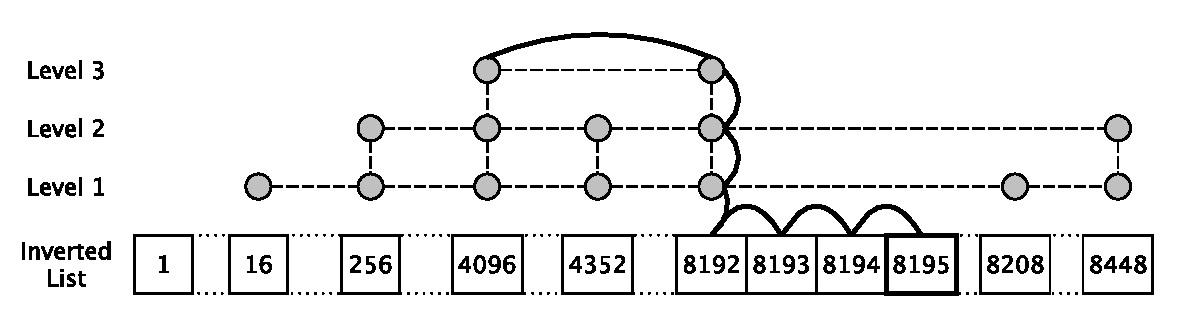
\includegraphics[scale=1]{pics/skiplists}
}%
\caption{Skip Lists with $p=\frac{1}{16}$. Dashed lines denote pointers between
synchronization points. The solid line shows the search path to the record 8195.}
\label{fig:skiplists}
\end{figure}

\section{Implementation}
 
 In this section we present the implementation of the Skip Lists structure as
 found in the open source project Apache Lucene\footnote{Apache Lucene:
 \url{http://lucene.apache.org/}}.
 
\paragraph{Structure}

The structure's data is kept on disk, and as such its implementation is done so
that the cost of IO operations are reduced. Each level of the Skip Lists is
stored as one stream, in order to read continuous data on disk when reading
synchronization points at a same level. The levels are stored one after the
other in reverse order, starting from the top level to level 1. The reverse
order storage of the levels is so that it maps the search algorithm flow, i.e.
we start on the top level, then descend levels to the bottom. The
Figure~\ref{fig:skiplists-impl} depicts the Skip Lists' Lucene implementation
of a synchronization point with 3 levels. The $ID$ refers to the record
identifier needed to advance in the Skip Lists. The \emph{Data} holds
information about the inverted list built upon such as file pointers. For a
same synchronization point such as in the figure, the Data block stores the same
information at each level about the inverted lists (i.e., duplicate data). The
next grey block depicts a file pointer, intern to the Skip Lists. This file
pointer stores the offset of a same synchronization point at the level below.
We can point out that for performance reasons, this file pointer points to the
end of a Data block, so that a duplicate information is not read twice when
descending levels.
 
\begin{figure}
\centering
\resizebox{0.6\linewidth}{!}{%
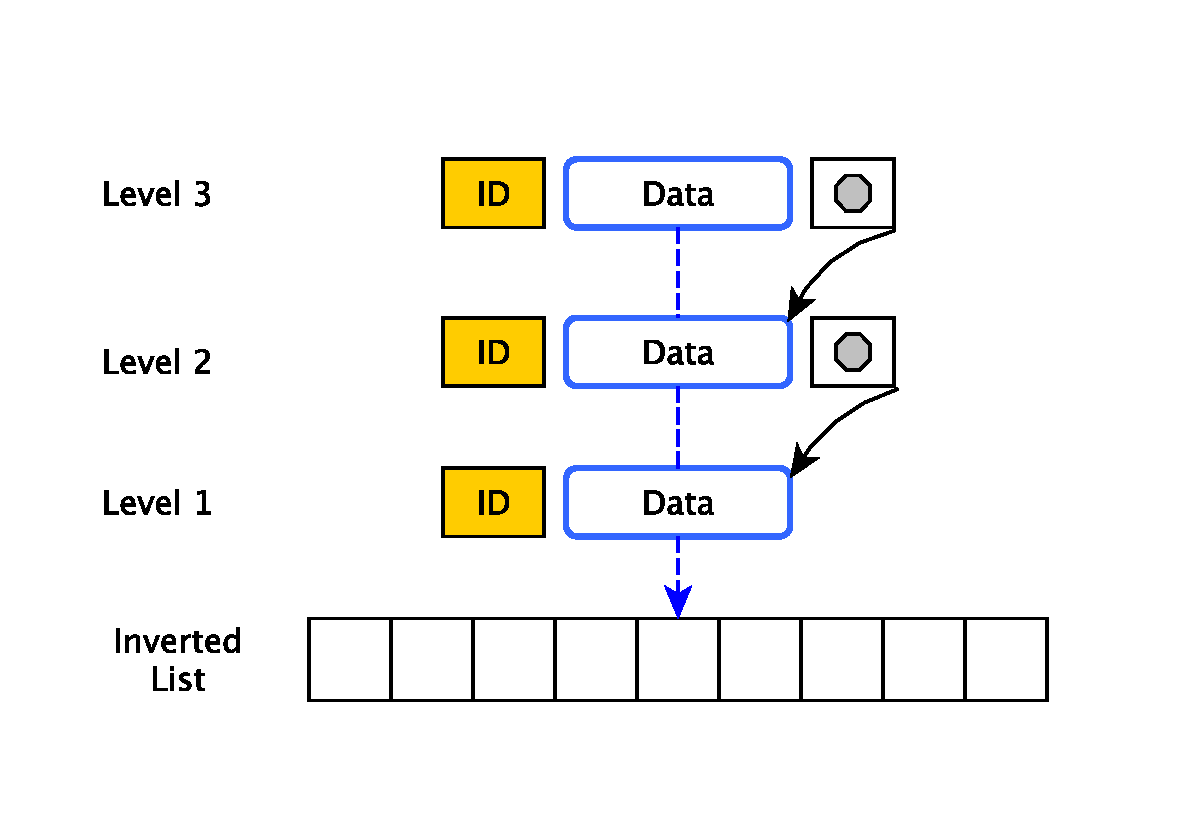
\includegraphics[scale=1]{pics/skiplists-impl}
}%
\caption{Skip Lists structure's implementation.}
\label{fig:skiplists-impl}
\end{figure}

\paragraph{Search algorithm}

The algorithm flow of the Skip Lists is highly optimized by having the less
branching conditions possible in order to maximizes the search throughput.
Given a targeted record that possibly is in the inverted list, the
\emph{\texttt{\#skipTo()}} method returns the interval that would hold it. On
the second line, the levels streams are loaded from disk if not done already.
The lines 4 to 6 walks up the levels as long as the current record identifier
of level i (i.e., stored within the \emph{currentIDs} variable) is lower than
the target. This allows to read only the levels that might skip to the target.
The loop starting at line 8 advances within the Skip Lists, by reading a
synchronization point at level i (line 10) as long as the current identifier is
lower than the target. On lines 12-13 we advance on the stream below to the
synchronization point which is the last being lower than the target.

\vspace{1em}
\begin{lstlisting}[frame=lines,language=Java,numbers=left,caption=Implementation of
the Skip Lists search
algorithm,label=lst:skiplists-search-algo,emph={currentIDs,moveToSynchronizationPoint,readSynchronizationPoint},
emphstyle={\bfseries}]
skipTo(int target)
	loadLevels();
	// Walk up the levels
	int level = 0;
	while (level < MAX_LEVELS - 1 && target > currentIDs[level + 1])
		level++;
	// Search for the interval containing the targeted record
	while (level >= 0) {
		if (target > currentIDs[level])
			readSynchronizationPoint(level)
		else
			moveToSynchronizationPoint(level-1);
			level--;
	}
\end{lstlisting}

